\chapter{Method}
\label{Method}
The flow diagram in figure \ref{fig:network} outlines IoT test bed constructed for this project. IoT devices pull power from the outlets through the smart switches. Smart switches log the power usage, and the WAP will query the smart switches for that data and pushes it to an AWS MySql database as an entry in the 'power' table. The IoT devices will also use the wireless network for general operation.

The wireless net provided through the WAP intercepts the network packets, parses them, splits them into power and network entries, and pushes them to the database as an entry in the 'ip\_log' table. Finally, for analysis, a second python script called realTimeGrapher.py pulls from the database and graphs this data in real time or from set intervals in the past.

The following sections discuss what devices we used, the set up of each device, and the physical layout of the IoT test bed. In the next section, the paper will go over the software part of the IoT test bed. Finally, the paper covers the usage flow of this test bed and what was done to obtain results for analysis.

\begin{figure}[H]
    \centering
    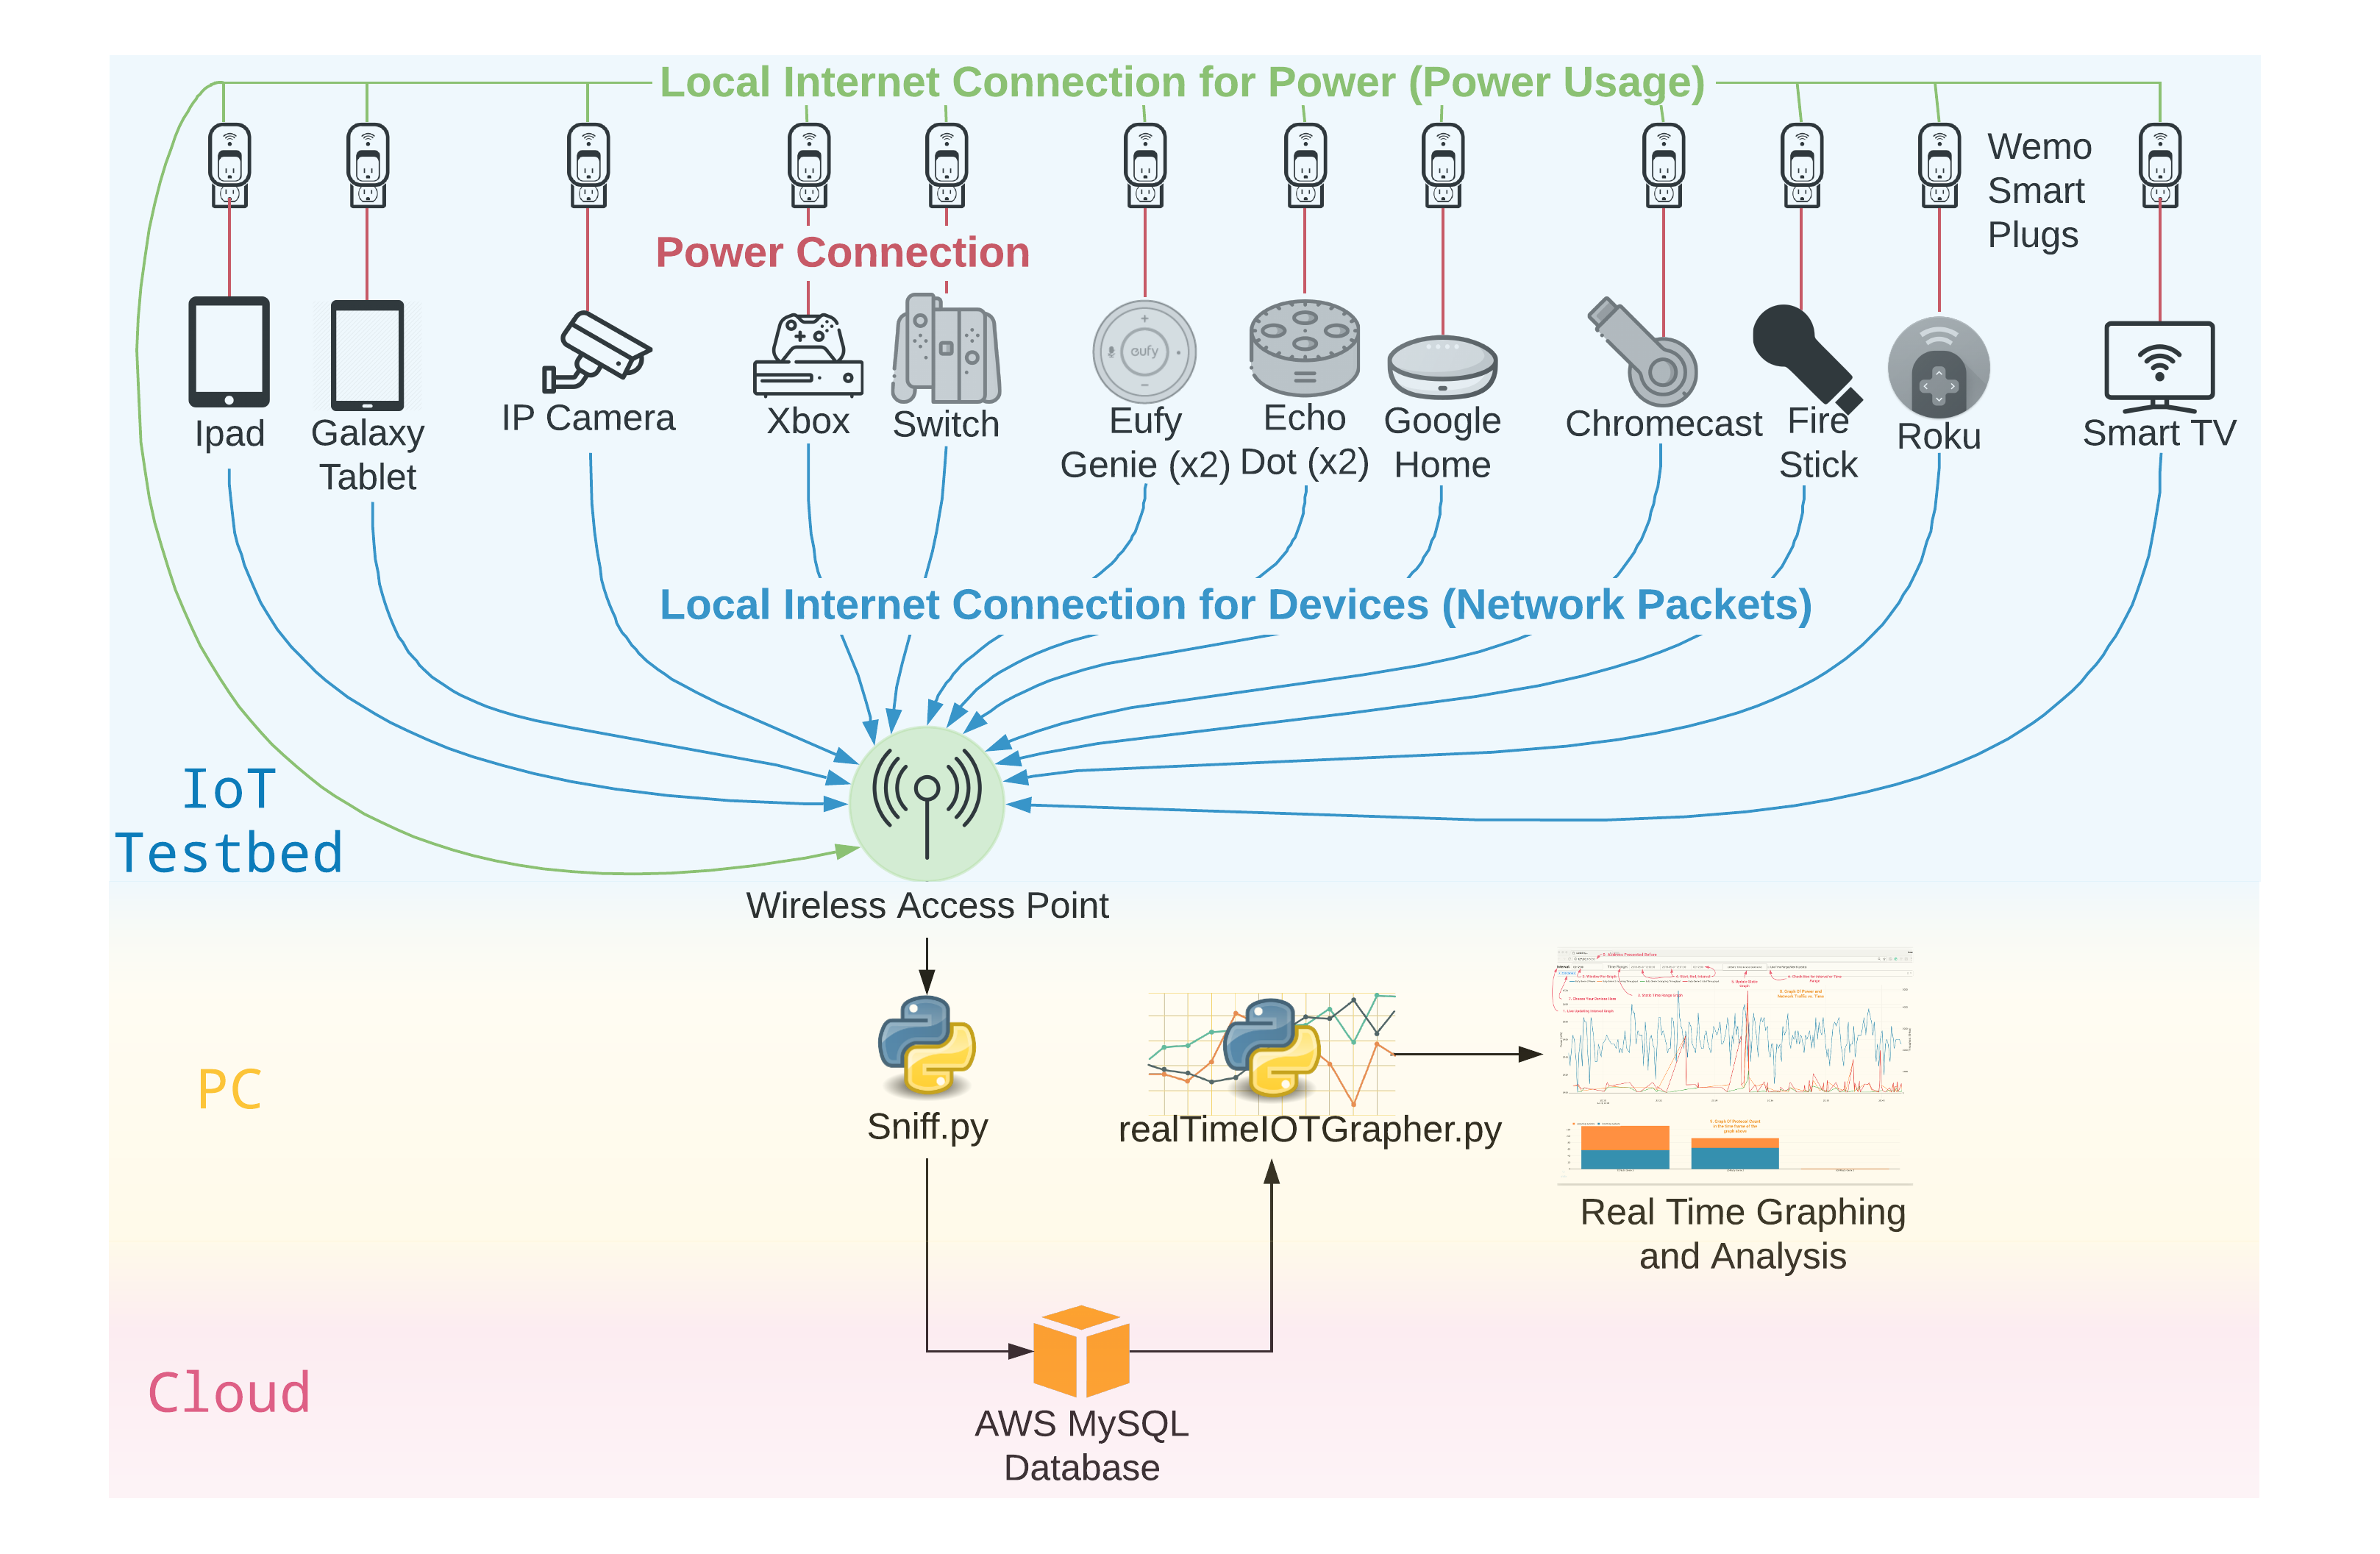
\includegraphics[width=1.0\textwidth]{networkDiagram}
    \caption{Network Diagram}
    \label{fig:network}
\end{figure}

\begin{figure}[H]
    \centering
    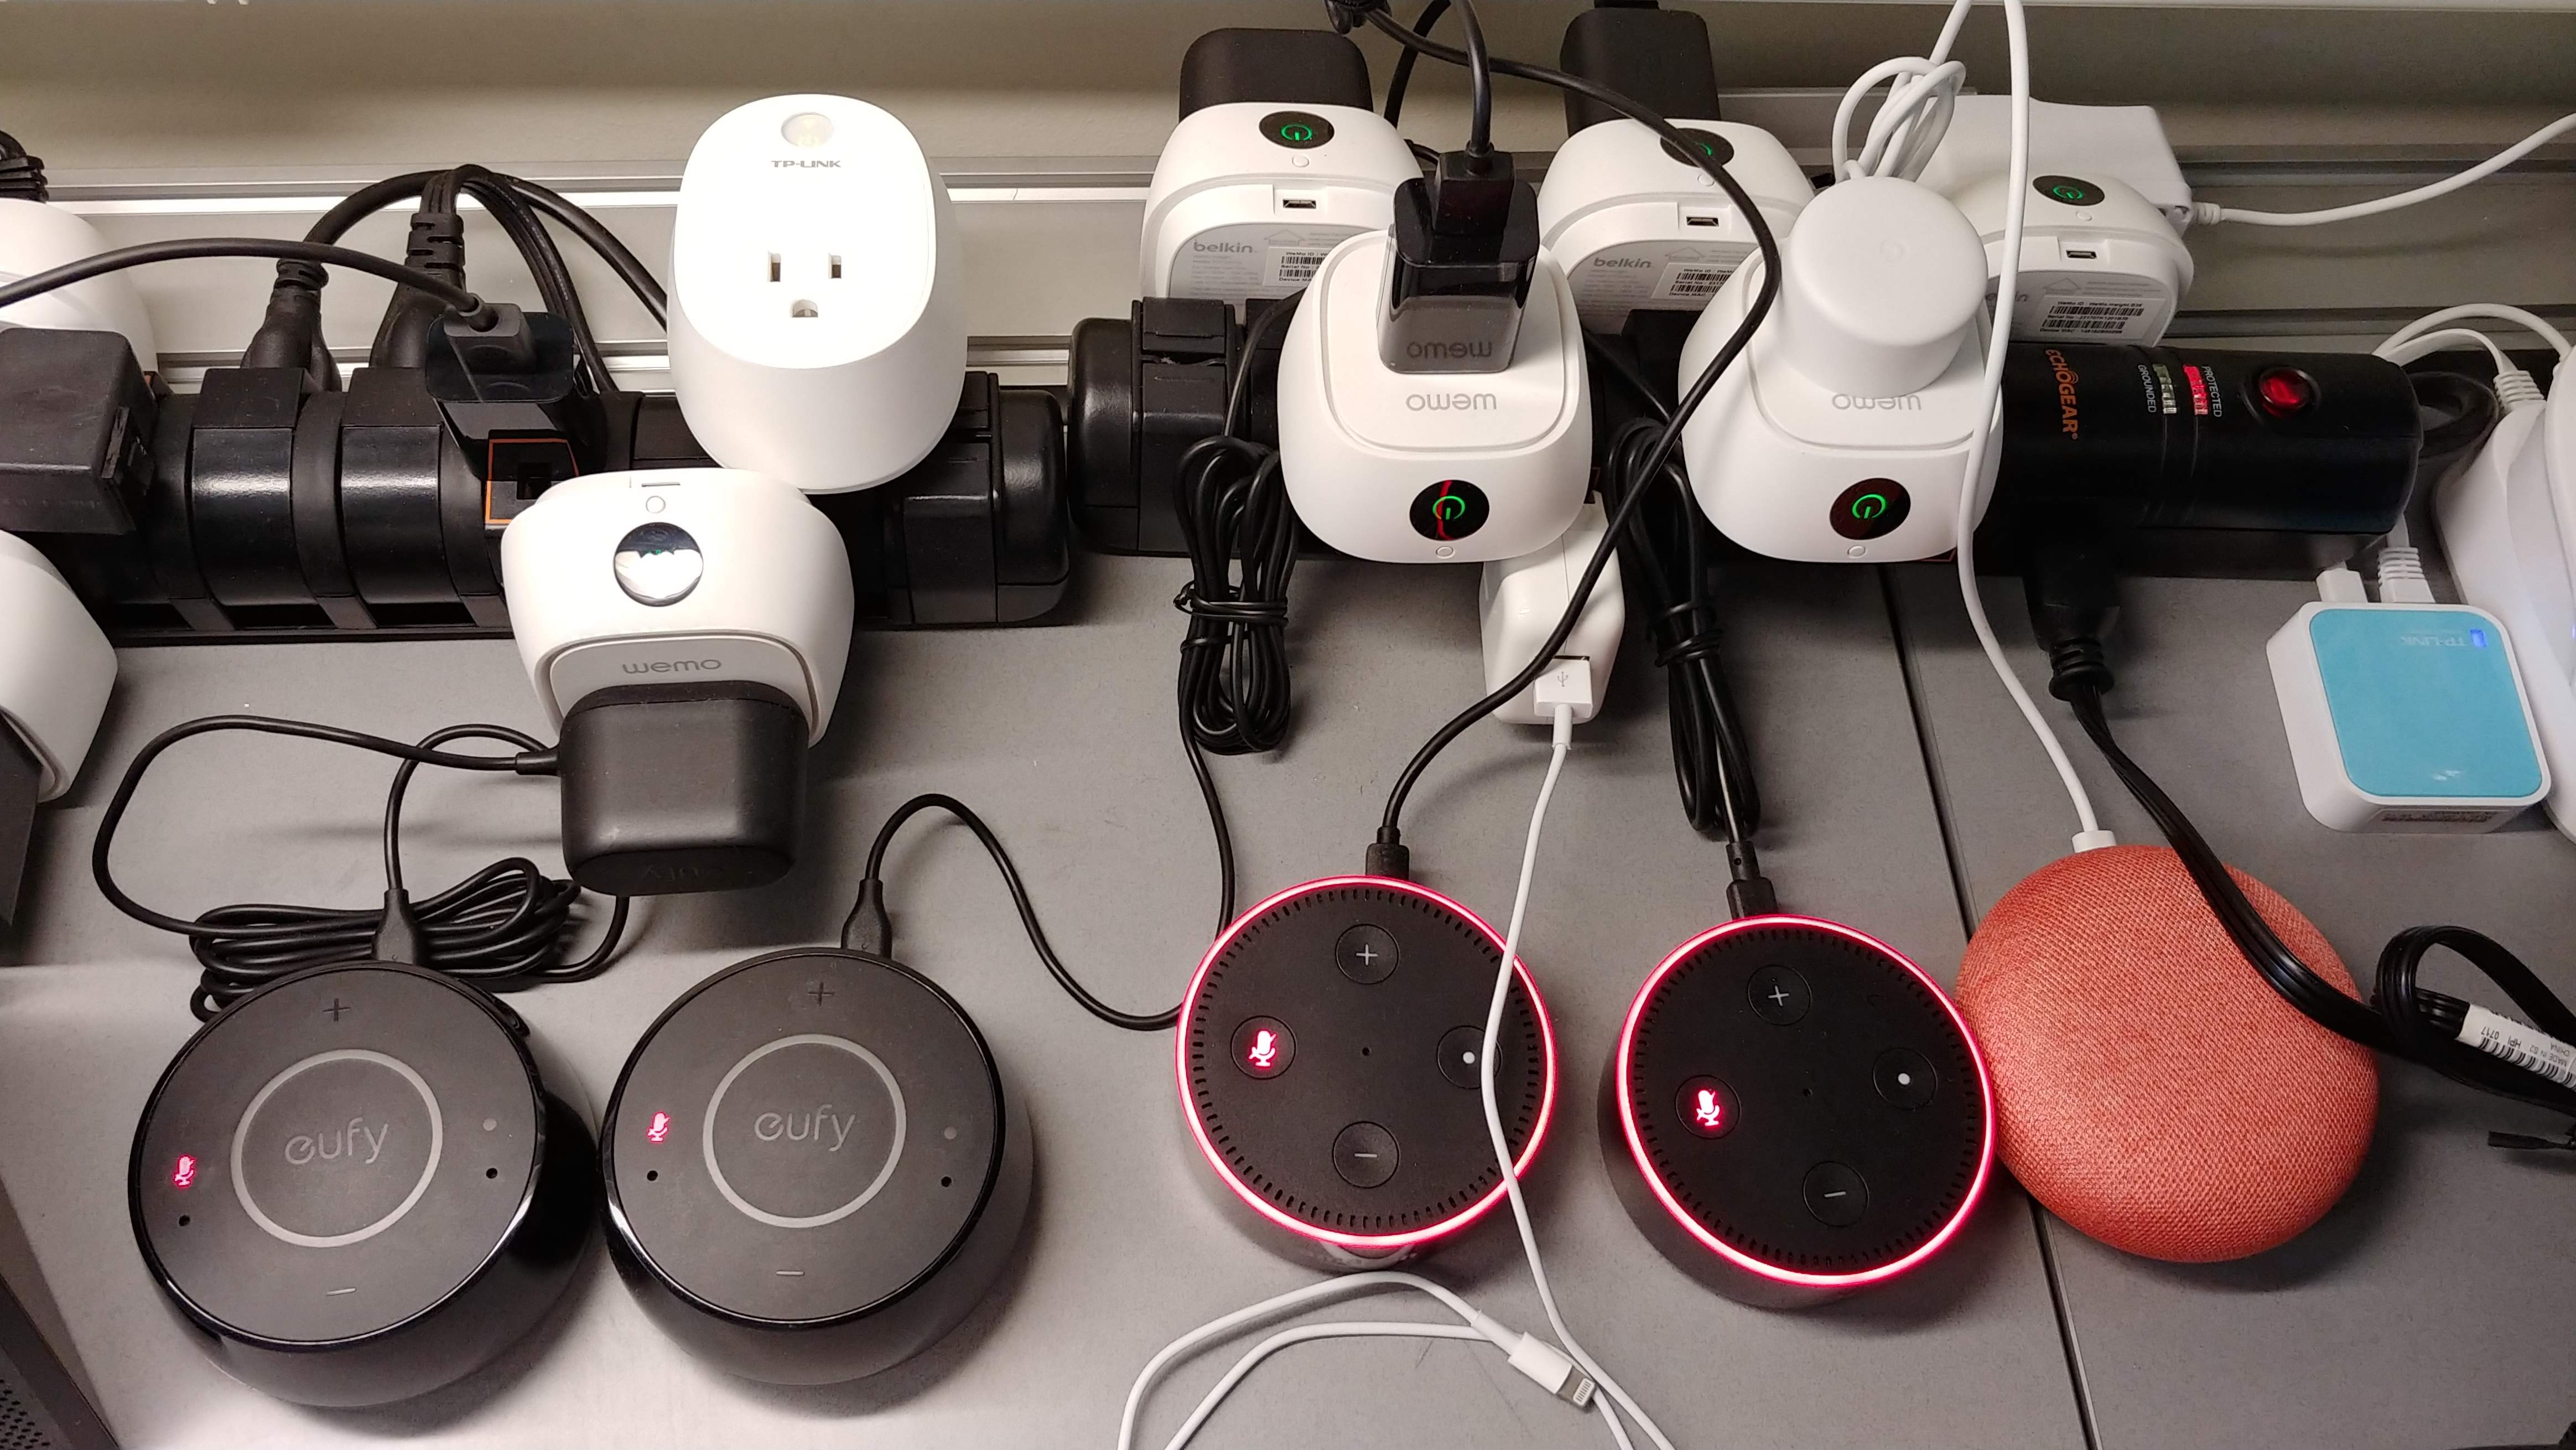
\includegraphics[width=1\textwidth]{wemos}
    \caption{Smart Speakers Connected to Wemo Insight Switches}
    \label{fig:wemo}
\end{figure}

\begin{figure}[H]
    \centering
    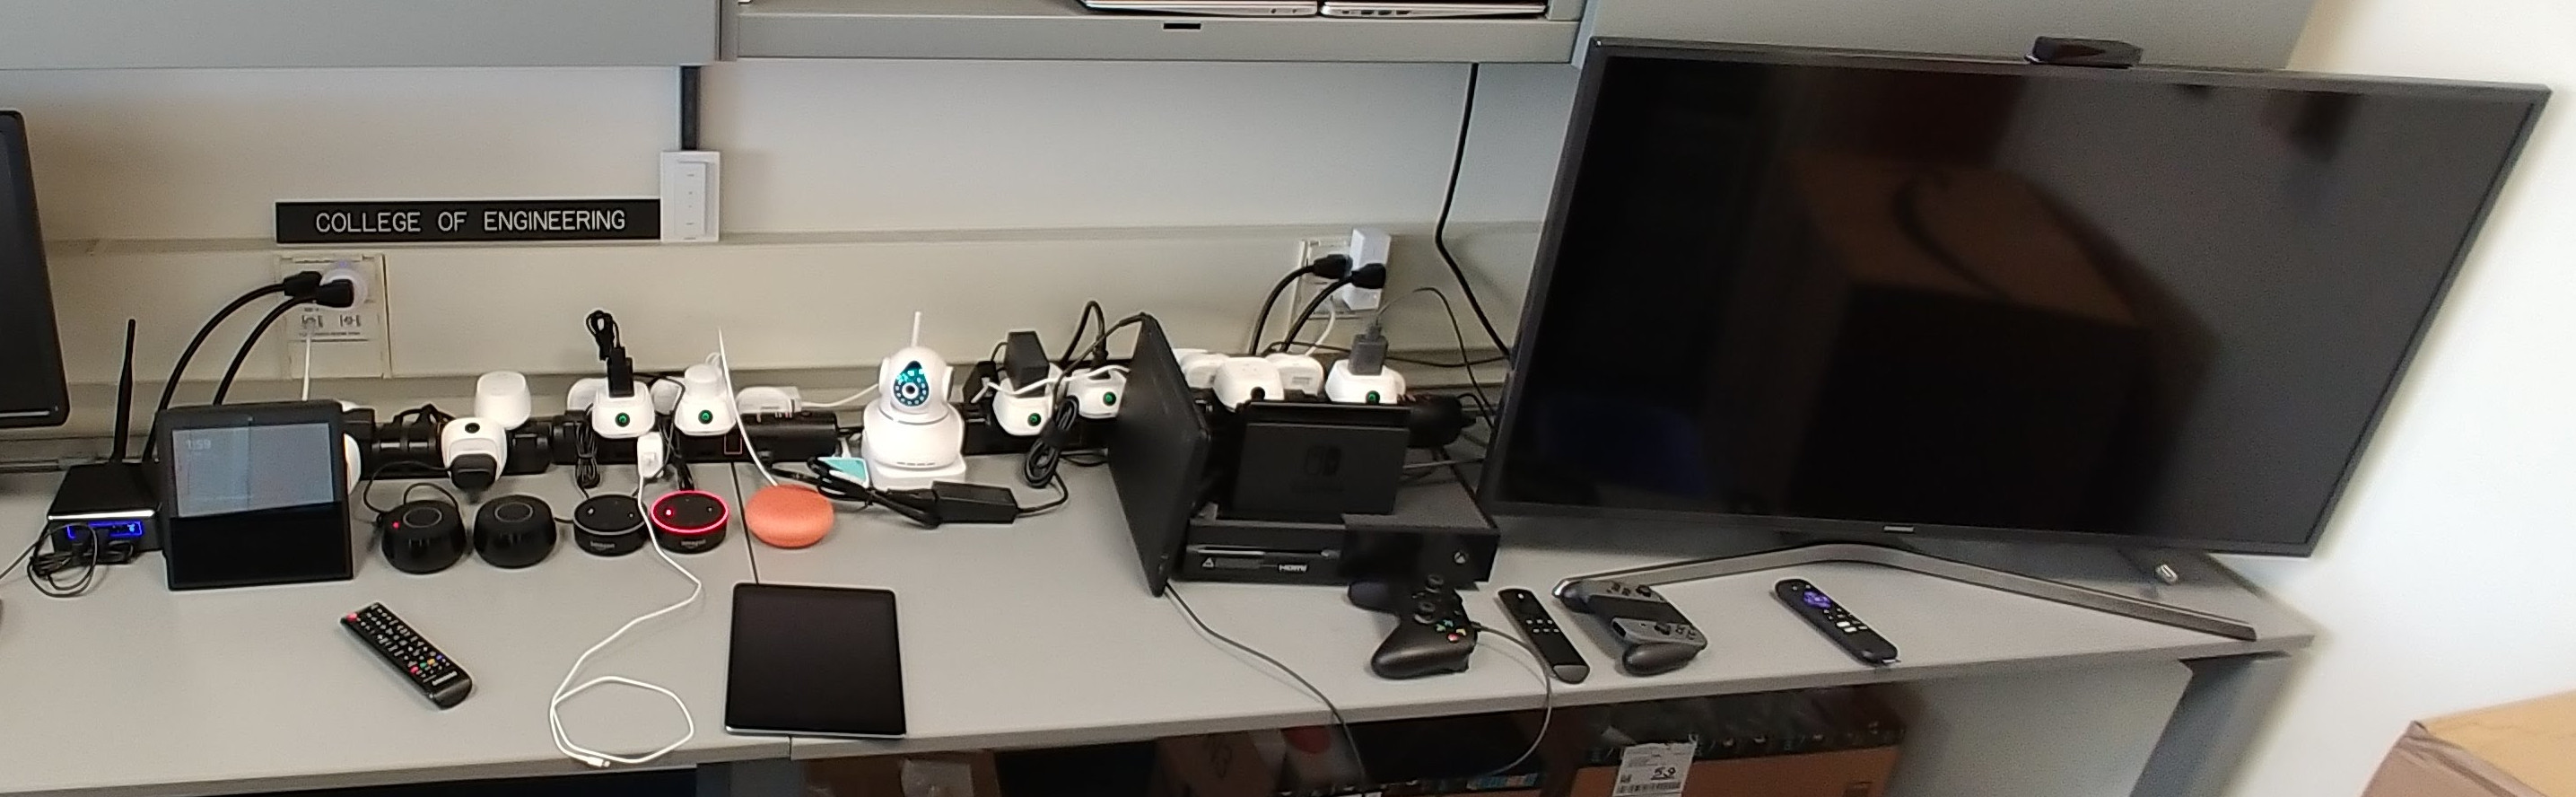
\includegraphics[width=1\textwidth]{devices}
    \caption{IoT Devices Under Examination}
    \label{fig:devices}
\end{figure}

\section{Physical Layout and set up}
\label{Physical Layout and set up}

This section covers the physical set up and layout of the hardware utilized when setting up the IoT test bed, the IoT devices we tested, and how each device is set up. Figures \ref{fig:wemo} and \ref{fig:devices} shows the IO testbed set up.

\subsection{Wireless Access Point}
\label{Wireless Access Point}
The wireless access point is an Intel NUC. We loaded Ubuntu on it because its the most common Linux OS and most flexible for developing scripts and programs to log network packets, query power information, and push those values to a database.

One challenging thing about the NUC is that its internal wireless chip is very slow. The throughput when using the wireless chip was measured to be 12 Mb/s down on Speedtest.net by Ookla when connected to with a chrome book (25 Mb/s is the minimum possible for broadband). This rate limitation caused many of the Wemos to drop their connection intermittently, causing gaps in recorded power data. To solve this, we added a USB wireless antenna to the NUC. This antenna improved our internet speed to 30 Mb/s down when tested on Speedtest.net by Ookla with the same chrome book, solving the issue where devices would drop their network.

\subsection{Devices}
\label{Devices}
This section goes over all the devices tested by groups, grouped by similar functionality. We grouped devices as smart speakers, streaming devices, video game consoles, tablets, security cameras, or other devices as listed in figure \ref{tab:devices}. These groups and devices were chosen based on their popularity, as the goal of the paper is to build a data set from common household IoT items and represent the average consumer.

\begin{table}[H]
    \centering
    \caption{IoT Devices Being Monitored}
    \begin{tabular}{@{}llll@{}}
    \toprule
    Category & Manufacturer & Device        & Quantity \\ \midrule
    Game Console & Nintendo     & Switch        & 1        \\
    Game Console & Microsoft    & Xbox One      & 1        \\
    Laptop & HP           & Chromebook    & 1        \\
    Media Player & Samsung      & Smart TV      & 1        \\
    Media Player & Google       & Chromecast    & 1        \\
    Media Player & Amazon       & Fire TV Stick    & 1        \\
    Media Player & Roku         & Express       & 1        \\
    Security Camera & Eray    & Hi3518 WiFi Camera     & 1        \\
    Smart Speaker & Amazon       & Echo Dot      & 2        \\
    Smart Speaker & Eufy/Anker   & Genie         & 2        \\
    Smart Speaker & Amazon       & Echo Show     & 1        \\
    Smart Speaker & Google       & Home Mini     & 1        \\
    Tablet & Amazon       & Fire 7 Tablet & 2        \\
    Tablet & Samsung      & Galaxy Tablet & 1        \\
    Tablet & Apple        & iPad          & 1        \\ \bottomrule
    \end{tabular}
    \label{tab:devices}
\end{table}

\subsubsection{Smart Speakers}
\label{Smart Speakers}

Smart speakers are IoT devices that combine speakers with built-in voice assistants, such as Amazon Alexa, Google Assistant, or Apple's Siri. These devices have limited physical button control that includes a mute, volume control, and a utility button. These devices are mainly controlled by voice commands, preceded by a wake word such as "hey Google".

Currently, around 39 million people (16 percent of the US population) use smart speaker\cite{perez_2017}. It is one of the top-selling IoT devices and is often a controller for smart homes because it can act a central voice control for everything. In 2022 it is projected that 70 million US households will have at least one smart speaker (55 percent of US households) and around 175 million smart speakers total\cite{perez_2018}. For these reasons, we included this group of devices in our research.

Within the smart speaker category, we included the Amazon Echo Dot, Google Home, and Eufy Genie. The Amazon Echo dot and the Google Home are the two leading smart speaker products. We added the Eufy Genie on because it is a third party Amazon Alexa device that we can compare with the Echo Dot. We also included the Amazon Show, which is a voice assistant with a screen.

\subsubsection{Streaming Devices}

Streaming devices are IoT products that connect to a television or built into a television (smart TVs) and streams videos or music from online services. In 2017 it was recorded that 70 million US households (58.7 percent of homes) had a television connected to streaming devices \cite{lynch_2017}. Netflix users collectively watched 1 billion hours of content per week in 2017 \cite{matney_2017}.

The specific streaming devices we look at include the Roku Express, Amazon Fire TV, and the Google Chromecast. These devices make up the three brands (Roku, Google Chromecast, Amazon Fire TV) that have a combined user base of over 110 million users who watch content at least once a month \cite{emarketer_2017}. For this reason, we selected these three devices for our studies.

To view content from these streaming devices, we use a Samsung smart TV. This TV also as streaming capabilities.

\subsubsection{Video Game Consoles}

Video game consoles are systems that were initially built specifically to play video games. We use 2 out of the three most popular gaming devices including the Nintendo Switch which sold 17.8 million units \cite{nintendo} and the Xbox One, which sold 30 million units \cite{souppouris_2016} as of January 2018.

\subsubsection{Tablets}

Tablets are devices that have phone operating systems running on them such as the Apple IPad, Samsung Galaxy tablet, and the Amazon Fire tablet. Ultimately these devices were mainly used for interacting with the other IoT devices since most of them require a smartphone or tablet for set up or control. Some of the IoT devices are also limited to either Android, which runs on the Galaxy, or IOS, which runs on the IPad, so we got both.

\subsubsection{Security Camera}

Security cameras are cameras meant to run constantly as surveillance, streaming the video footage a user can view from any connected device at all times. Two out of the five largest recorded cybersecurity attacks targeted security cameras \cite{guest_2018}. The specific camera we use is the Eray camera. It is a generic Alibaba device with a weak username:password of admin:1234. A weak username and password makes it very susceptible to cyber attacks. There have also been reports that smart cameras have been found to send unencrypted data \cite{feamster_2016}. Because this device is a third party, unknown manufacturer, this device is an outlier for which we hope to get more interesting data.

\subsubsection{Other Devices}

We also connected several other devices that are harder to categorize.

We have a smart hub connected to a smart lock, an indoor room temperature sensor, and smart LED light bulbs. These devices are difficult to analyze because they communicate with the smart hub through Zigbee or Bluetooth at which point the smart hub aggregates the data and communicates with the network. In order to look at the network traffic caused by smart lights individually, we prevented all devices besides the smart LED bulbs from communicating with the smart hub. This isolation minimized other packet noise to the smart hub so that we can monitor the smart hub traffic as a replacement for the smart LED bulbs. However, even then, the smart hub might have extra overhead for other tasks, making isolated analysis difficult.

We also have a Chromebook which we used to control the Chromecast. However, because this is more a laptop than an IoT device, we decided to leave this out during our research

\subsection{Smart Power Plugs}

Smart power plugs are WiFi capable, pass through outlets that a device plugs into. The outlets collect and transmit power states over the network. For this reason, they are critical to the power consumption logging in this research.

We used the Belkin Wemo. We chose this smart plug because there are many open source Python libraries for pulling power information from them and because they were the easiest to set up.

When setting these smart plugs up, we named each smart plug based on the device connected to it so that when we pull power information with our scripts, we can easily reference data to a smart plug. This informal naming leads to issues when the wrong device is connected to the wrong smart plug, as discussed in section \ref{realtimeIoTGrapher.py}

\subsection{Wiring and Configuration}

When setting up the smart plugs, we manually named each smart plug in reference to the device connected to it. We also tried to set static IPs for each device, but we decided that the average user would not set up a static IP for their device and left dynamic IPs.

The next step was to set up each device and corresponding smart plug through their set up application, filling in the devices, name, email, network configuration, and any other setup details.

When plugging in all of the devices for the first time for power, we worked to plug each device into the corresponding Wemo smart plug and connected to our WAP during device set up so that we could instantly log power and traffic information. It was essential to log power as soon as possible to catch data while a device is starting up. Some devices had already been opened and used, so they do not contain startup information(Xbox and the Echo Dot 1).

Set up and configuration took up a significant portion of the time. We worked to set up each device with a separate email account. To do this, we made around 20 AOL accounts. We wanted email addresses that were not under control of the manufacturer of any of the devices. For example, we did not want to use any Gmail accounts because we did not want the Google home or Google Chromecast do perform domain-specific optimizations. When setting up AOL accounts, we also faced a limitation of the number of email accounts tied to a single phone number. We had to use different phone numbers in order to circumvent this.

We set up each device in waves, taking around a week to set everything up. Incremental device setup with no plan resulted in a messy work environment, which made it difficult to match a device to it is corresponding smart plug. The Wemos also take up too much space to be plugged right next to each other. After a month of data logging, it was difficult to keep track of each device because we had not kept it organized. We unplugged everything, renamed the Wemos, organized the wiring, and organized the location of each smart device resulting in the set up in figure \ref{fig:devices} and \ref{fig:wemo}. With limited power strips, the organization helped maximize power ports. We also made sure to face the button for each power plug towards our view so that we can quickly notice whether the power plugs were on or off. Organization streamlined the logging process in the long run. Debugging network and connection issues was much simpler with an ordered set up. Now we could quickly identify each device and go down the line when running procedures on the devices.

\section{Software}
\label{software}
This section covers the software components used to control the IoT test bed. It includes the scripts for logging power and network traffic, the database information, and the python script for visually viewing the database.

\subsection{Wireless AP Code}
In order to turn the NUC into a wireless access point, we utilized a create\_ap script\cite{guest_2018}CITEoblique\_2017. This app takes in the WiFi name, WiFi password, and the wireless interface. This script turned the NUC into a wireless access point (WAP). We later found that, with newer versions of Ubuntu, there is a built-in feature for creating a hotspot through a wireless interface on the device\cite{guest_2018}CITEm\_2016. We later used this feature. Partially through our research, as we set up more IoT devices and demand for bandwidth through the WAP increased, we had to switch to an external antenna and rerun the script in order to set the USB antenna as the WAP wireless interface causing a void of traffic due to this switching.

\subsection{sniff.py}
\label{sniff.py}

Sniff.py is a python script that runs on the Intel NUC. It runs a thread for power logging and a thread for network logging. As each logger runs, it writes the network packets and power information to a MYSQL database hosted on AWS through the python mysqlclient library. If the database connection is lost, the script automatically reconnects.

\subsubsection{Network Logging}

Network logging is the largest part of the script with 180 lines of code out of 290. It begins by opening a socket on the wireless interfaces connected. All IP packets are sniffed through this socket connection as shown in listing \ref{lst:sock}.

\begin{lstlisting}[label={lst:sock},caption={Open and Read from a Socket},captionpos=b]
self.socket = socket.socket(socket.AF_PACKET, socket.SOCK_RAW, socket.htons(ETH_P_ALL))
self.socket.setsockopt(socket.SOL_SOCKET, socket.SO_RCVBUF, 2**30)
self.socket.bind((self.interface_name, ETH_P_ALL))
while True:
    packet, address = self.socket.recvfrom(MTU)
\end{lstlisting}

Once we have sniffed a packet, we can obtain the raw metadata in the form of a hex dump. We preserve the hex dump block because it is a raw, untouched packet. The fields we write to the database are the source IP, source host, destination IP, destination host, time, size, type, protocol, source port, destination port, source host, destination host, and hex dump. We will explain what each field in the database section.

\subsubsection{Power Logging}

The second addition to our IoT device analysis is the power information. To obtain this information, we rely heavily on the Belkin Wemos. Each Belkin Wemo Insight connects to an outlet and each IoT device plugs into the Wemos.

We used the PyWemo python script to read power usage form the Wemos once per second. However, this is the highest we were able to obtain. The Wemo is capable of reading both power and energy in mW and kW hours.

Once the script queries the Wemo for its power information, we relate the Wemo to the device connected to it by extracting the name of the Wemo. This information is used as well when pushing this data to our database.

One issue with PyWemo and the Belkin Wemo's was that they would sometimes disconnect and the script would miss out on power data. To solve this issue, the script rescans for Wemos until it finds all the Wemos. If it does not find the of Wemo's in our testbed (hardcoded value). The code for this is shown below in figure \ref{fig:wemoRescanCode}

\begin{figure}[H]
    \centering
    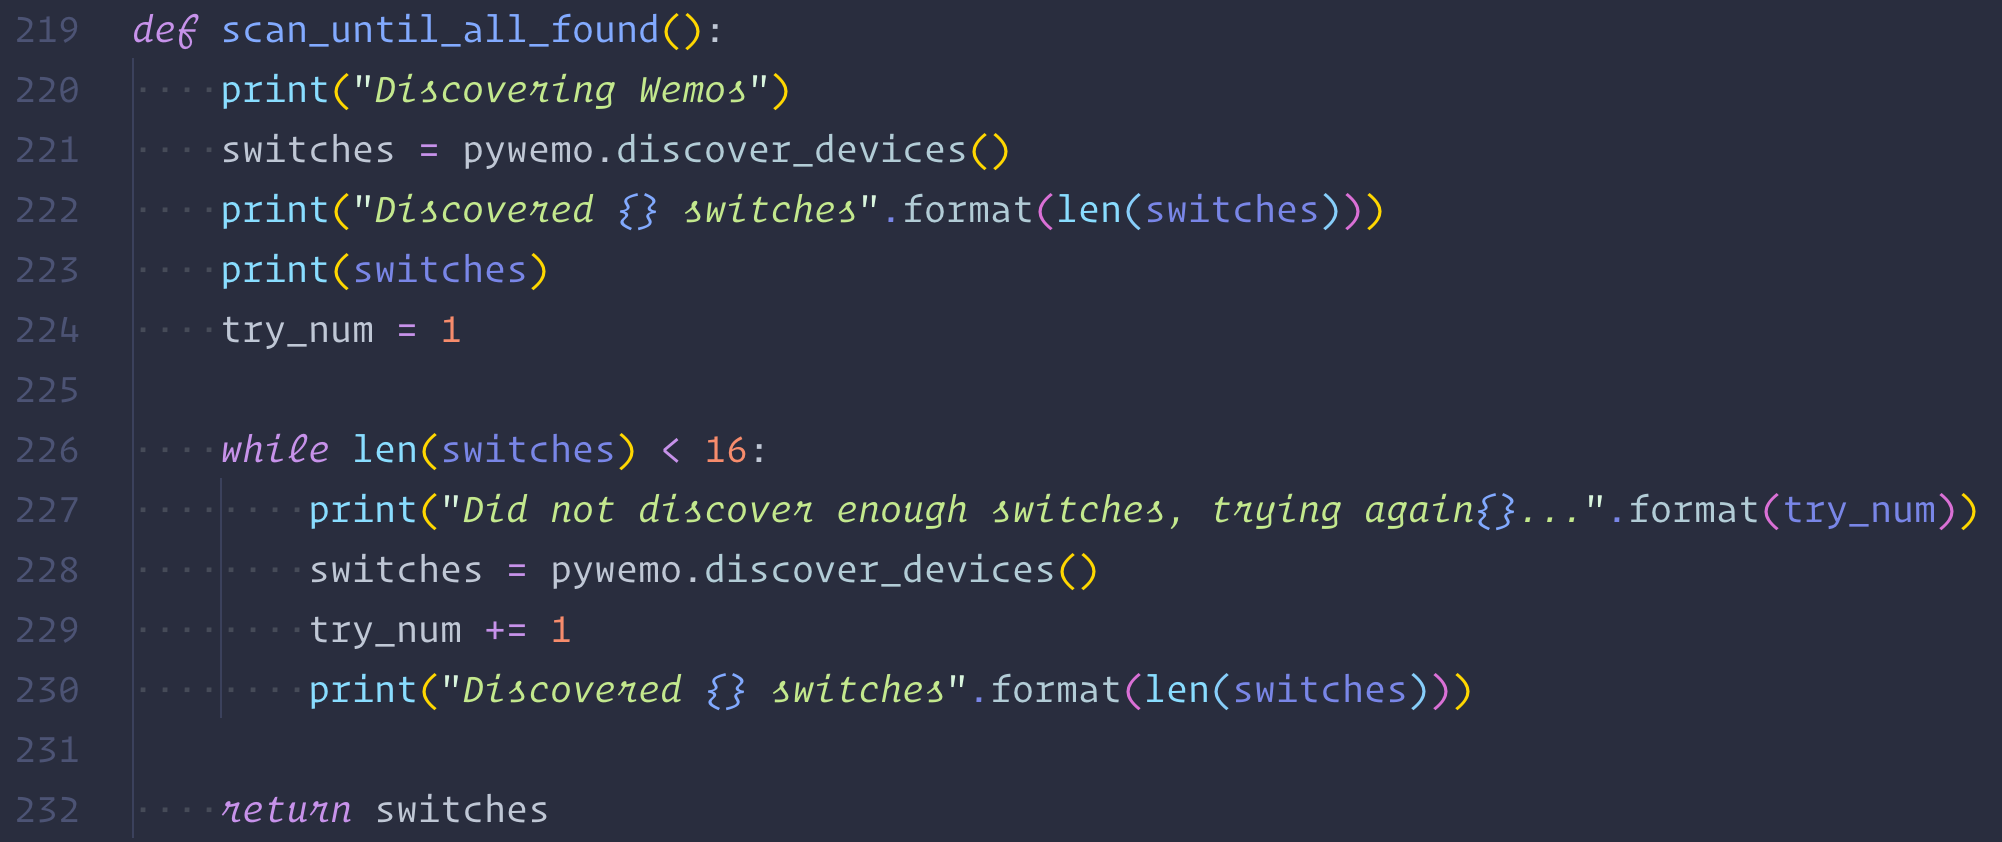
\includegraphics[width=1\textwidth]{figures/wemoRescanCode.png}
    \caption{Rescan if all wemos not found.}
    \label{fig:wemoRescanCode}
\end{figure}

\subsection{Database}
\label{Database}

To store all the result of the sniffed packets and power data, we push the data to a MySQL database hosted on an Amazon AWS server. As of writing this paper, the database currently holds 172,445,929 entries that take up 184.94 GB of space.

\subsubsection{Network Table}

The largest part of our database is the IP network table. This table contains all the network packets that have gone through the NUC WAP. It is currently 179.1 GB and contains 116830077 entries. It is so large because it consists of constant network packets through at least 12 months of research. In those 12 months, we did many high bandwidth tasks such as playing music or video. These entries also contain the raw hex dump of the whole packet, which contains all the metadata plus data load, further contributing to the massive size of this table. The data table's rows represent a single packet with the columns shown in the table below \ref{tab:netcol}.

\begin{table}[H]
    \centering
    \caption{Columns in Network Traffic Table}
    \begin{tabular}{@{}lll@{}}
    \toprule
    Column Number & Column Name & Data Type \\ \midrule
    1             & time        & datetime  \\
    2             & source      & varchar   \\
    3             & src\_host   & varchar   \\
    4             & destination & varchar   \\
    5             & dst\_host   & varchar   \\
    6             & protocol    & varchar   \\
    7             & type (in/out)       & varchar   \\
    8             & src\_port   & varchar   \\
    9             & dst\_port   & varchar   \\
    10            & size        & int       \\
    11            & hexdump     & longtext  \\ \bottomrule
    \end{tabular}
    \label{tab:netcol}
    \end{table}

With these columns, some common SQL commands we used for our analysis includes common queries shown in figures \ref{fig:navicatPowerQuery} and \ref{fig:navicatNetworkQuery}. The most useful commands generally required examining total throughput or device throughput. The SQL query shown in \ref{fig:navicatRollup}.

\begin{figure}[H]
    \centering
    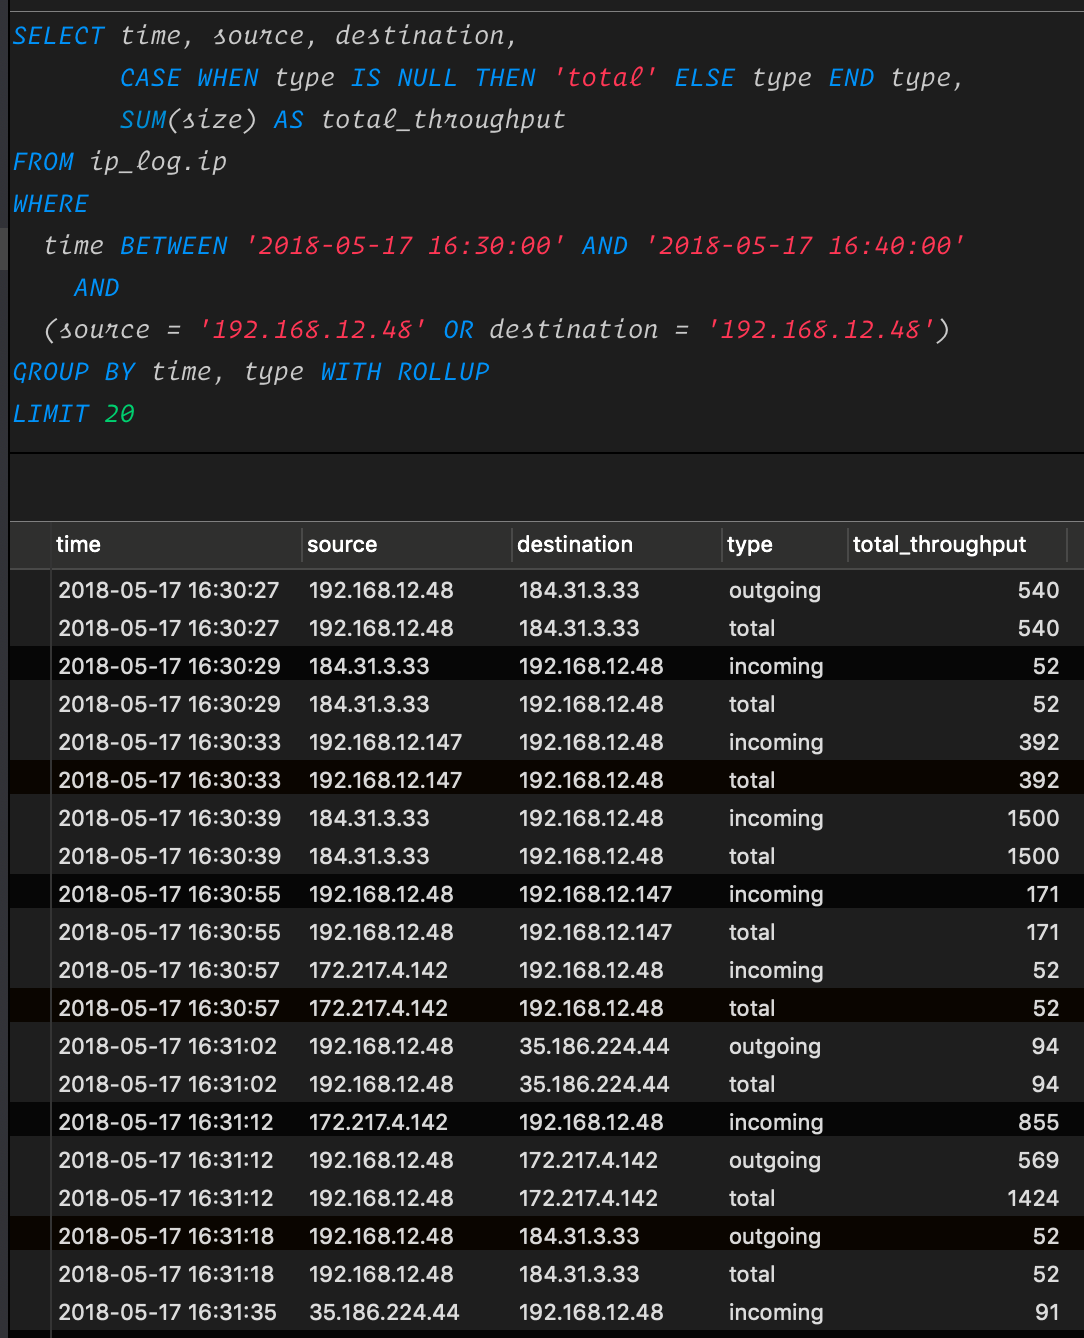
\includegraphics[width=1\textwidth]{figures/navicatRollup.png}
    \caption{Navicat ip query with rollup.}
    \label{fig:navicatRollup}
\end{figure}

The hex dump column drastically increases the size of each entry in the network table. However, as a raw network packet, it is very flexible and can be manipulated for many more use cases than the targeted columns we have. The hex dump contains the information of all the columns in the table and more. This flexibility is useful for other researchers who may have slightly different needs. As one of the original goals is to provide a database that other network researchers can use, the addition of the hex dump strongly hits that point

In the tables, each device can be tracked down by looking for the IP address of that device in the source or destination columns. However, note that during set up, we did not set up static IPs for these devices. Because of this, a single device can be under multiple IPs within the table. We ignored this issue until a query for a particular IP stopped working. At which point we would invoke a command on the device whose IP changed to flood the database with packets from that device, query the database in the time frame of the command, and obtain the new IP.

\subsubsection{Power Table}

The power table holds the most important data to this research, and we refer to it for the majority of the paper's findings. The size of this table is much smaller than the network table. It contains 5.84 GB of data and 61240189. The large difference in size between the IP table and power table is because each device only produces one entry power entry every second. The Power table is shown below in figure\ref {tab:powcol}.

\begin{table}[H]
    \centering
    \caption{Columns in Power Table}
    \begin{tabular}{@{}lll@{}}
    \toprule
    Column Number & Column Name     & Data Type \\ \midrule
    1             & name            & varchar   \\
    2             & power\_mw       & int       \\
    3             & time            & datetime  \\
    4             & today\_kwh      & varchar   \\
    5             & on\_for         & varchar   \\
    6             & today\_on\_time & varchar
    \end{tabular}
    \label{tab:powcol}
    \end{table}

When working with this database, we generally query for all the most recent power packets or a range of power packets in a given time range. We do this for either all devices, a subset of devices, or a single device. Some of the commands and results are shown below in figures \ref{fig:navicatPowerQuery} and \ref{fig:navicatNetworkQuery}.

\begin{figure}[H]
    \centering
    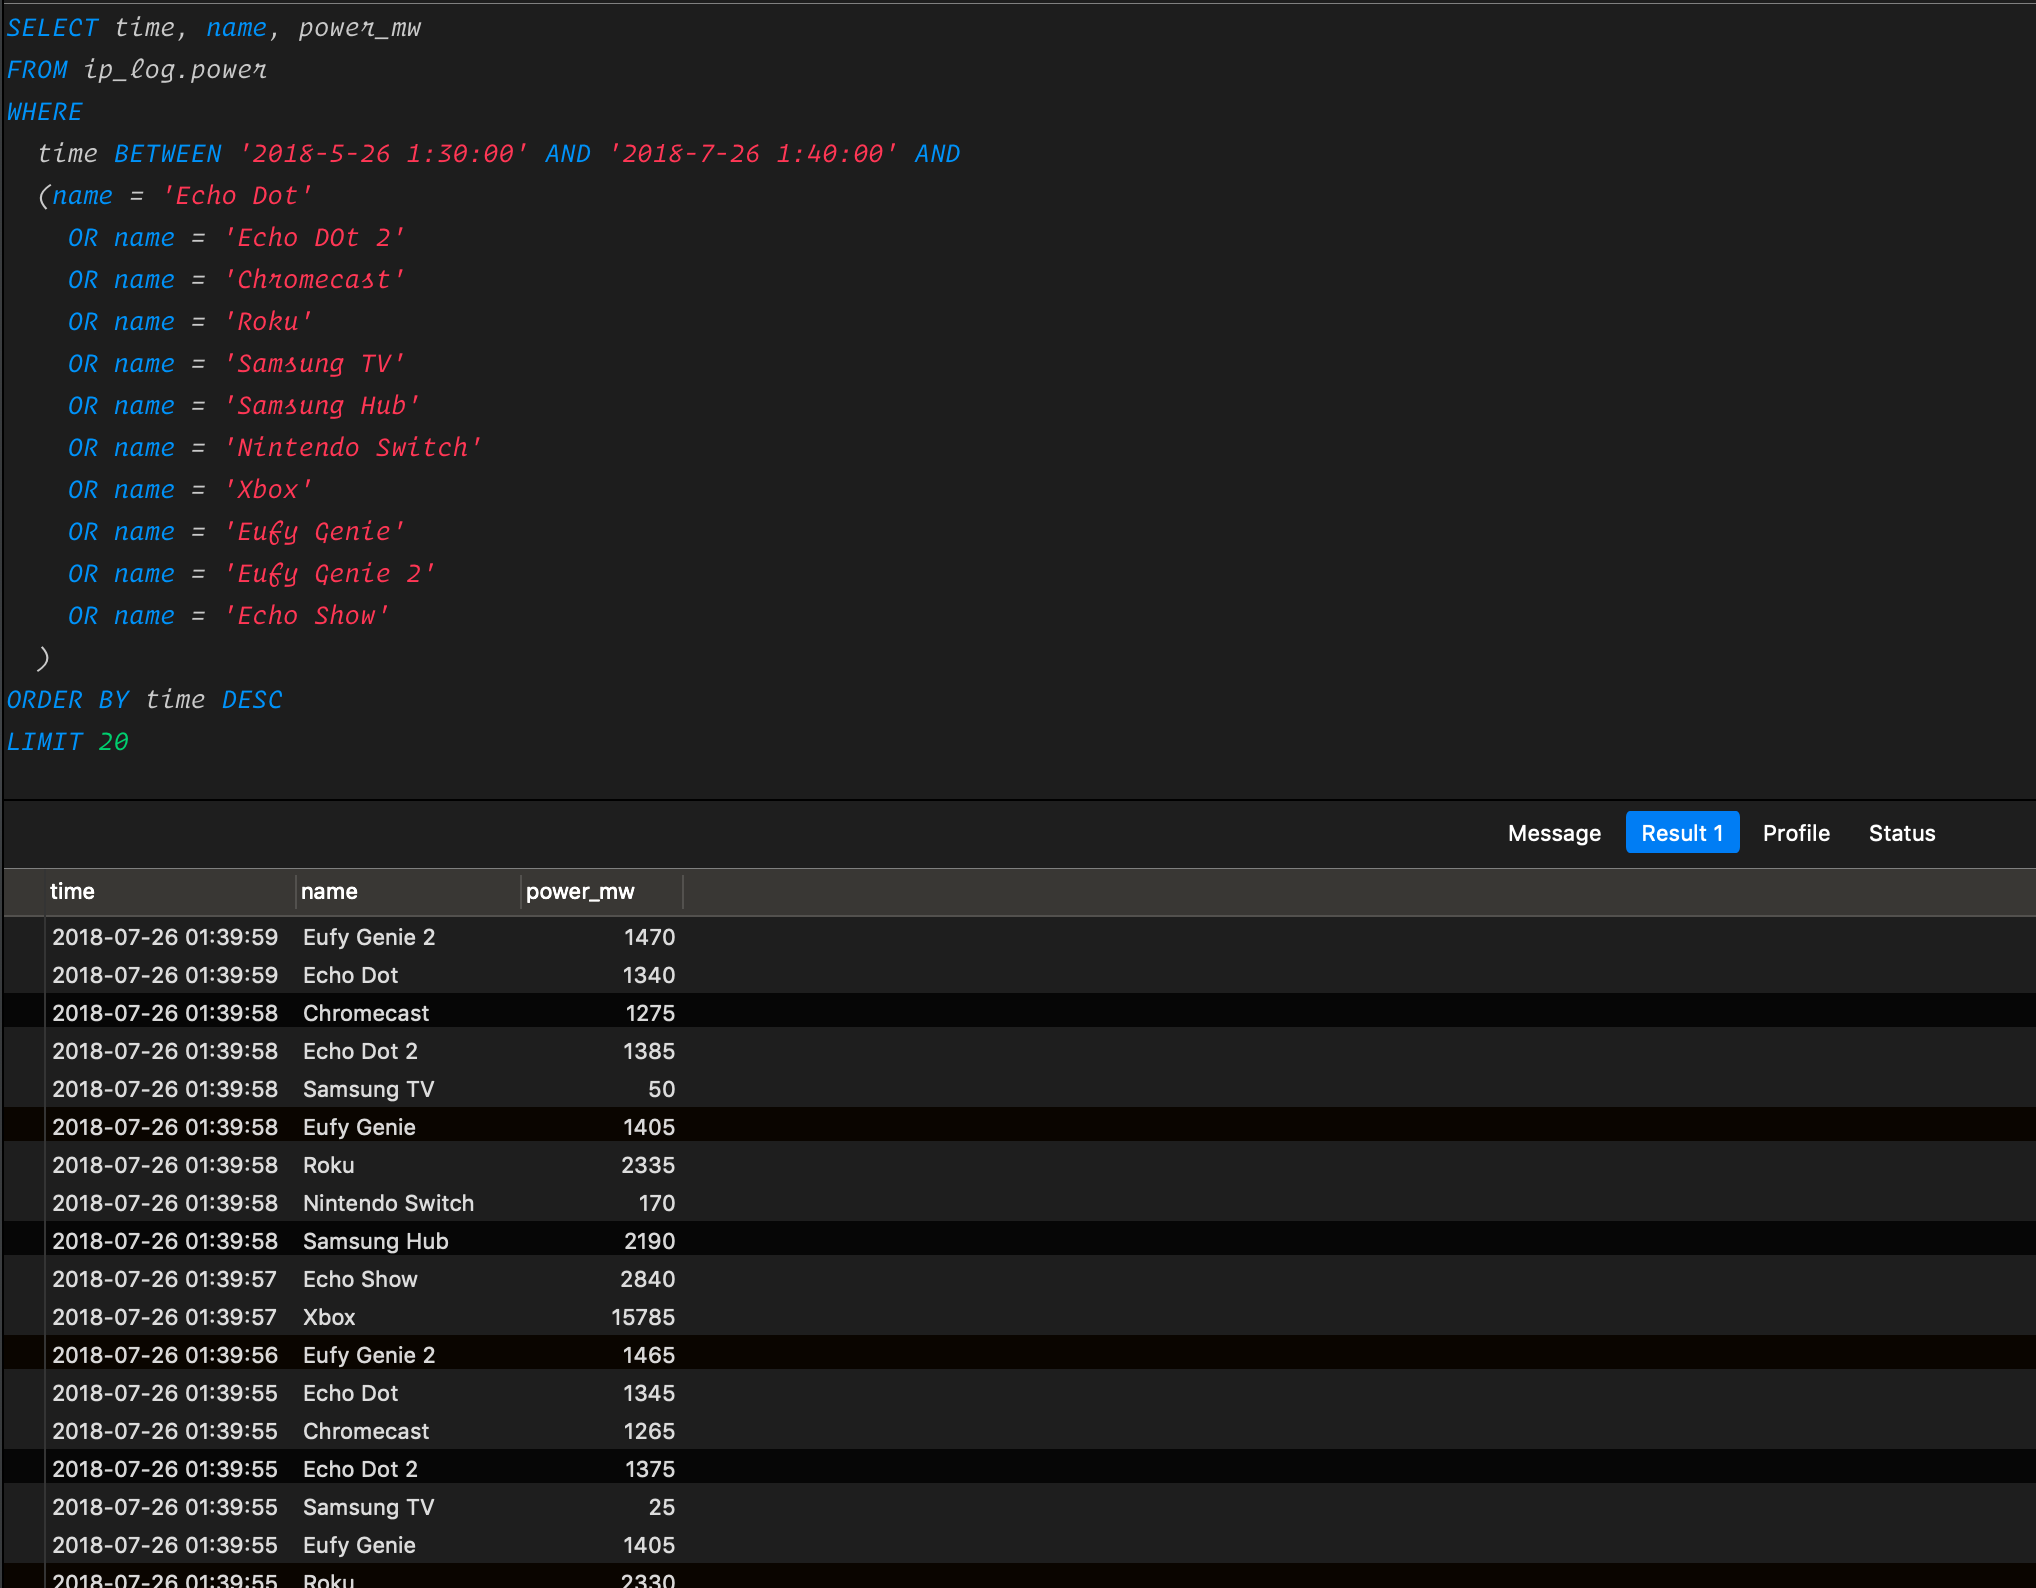
\includegraphics[width=1\textwidth]{figures/navicatPowerQuery.png}
    \caption{Power query form database with navicat.}
    \label{fig:navicatPowerQuery}
\end{figure}

\begin{figure}[H]
    \centering
    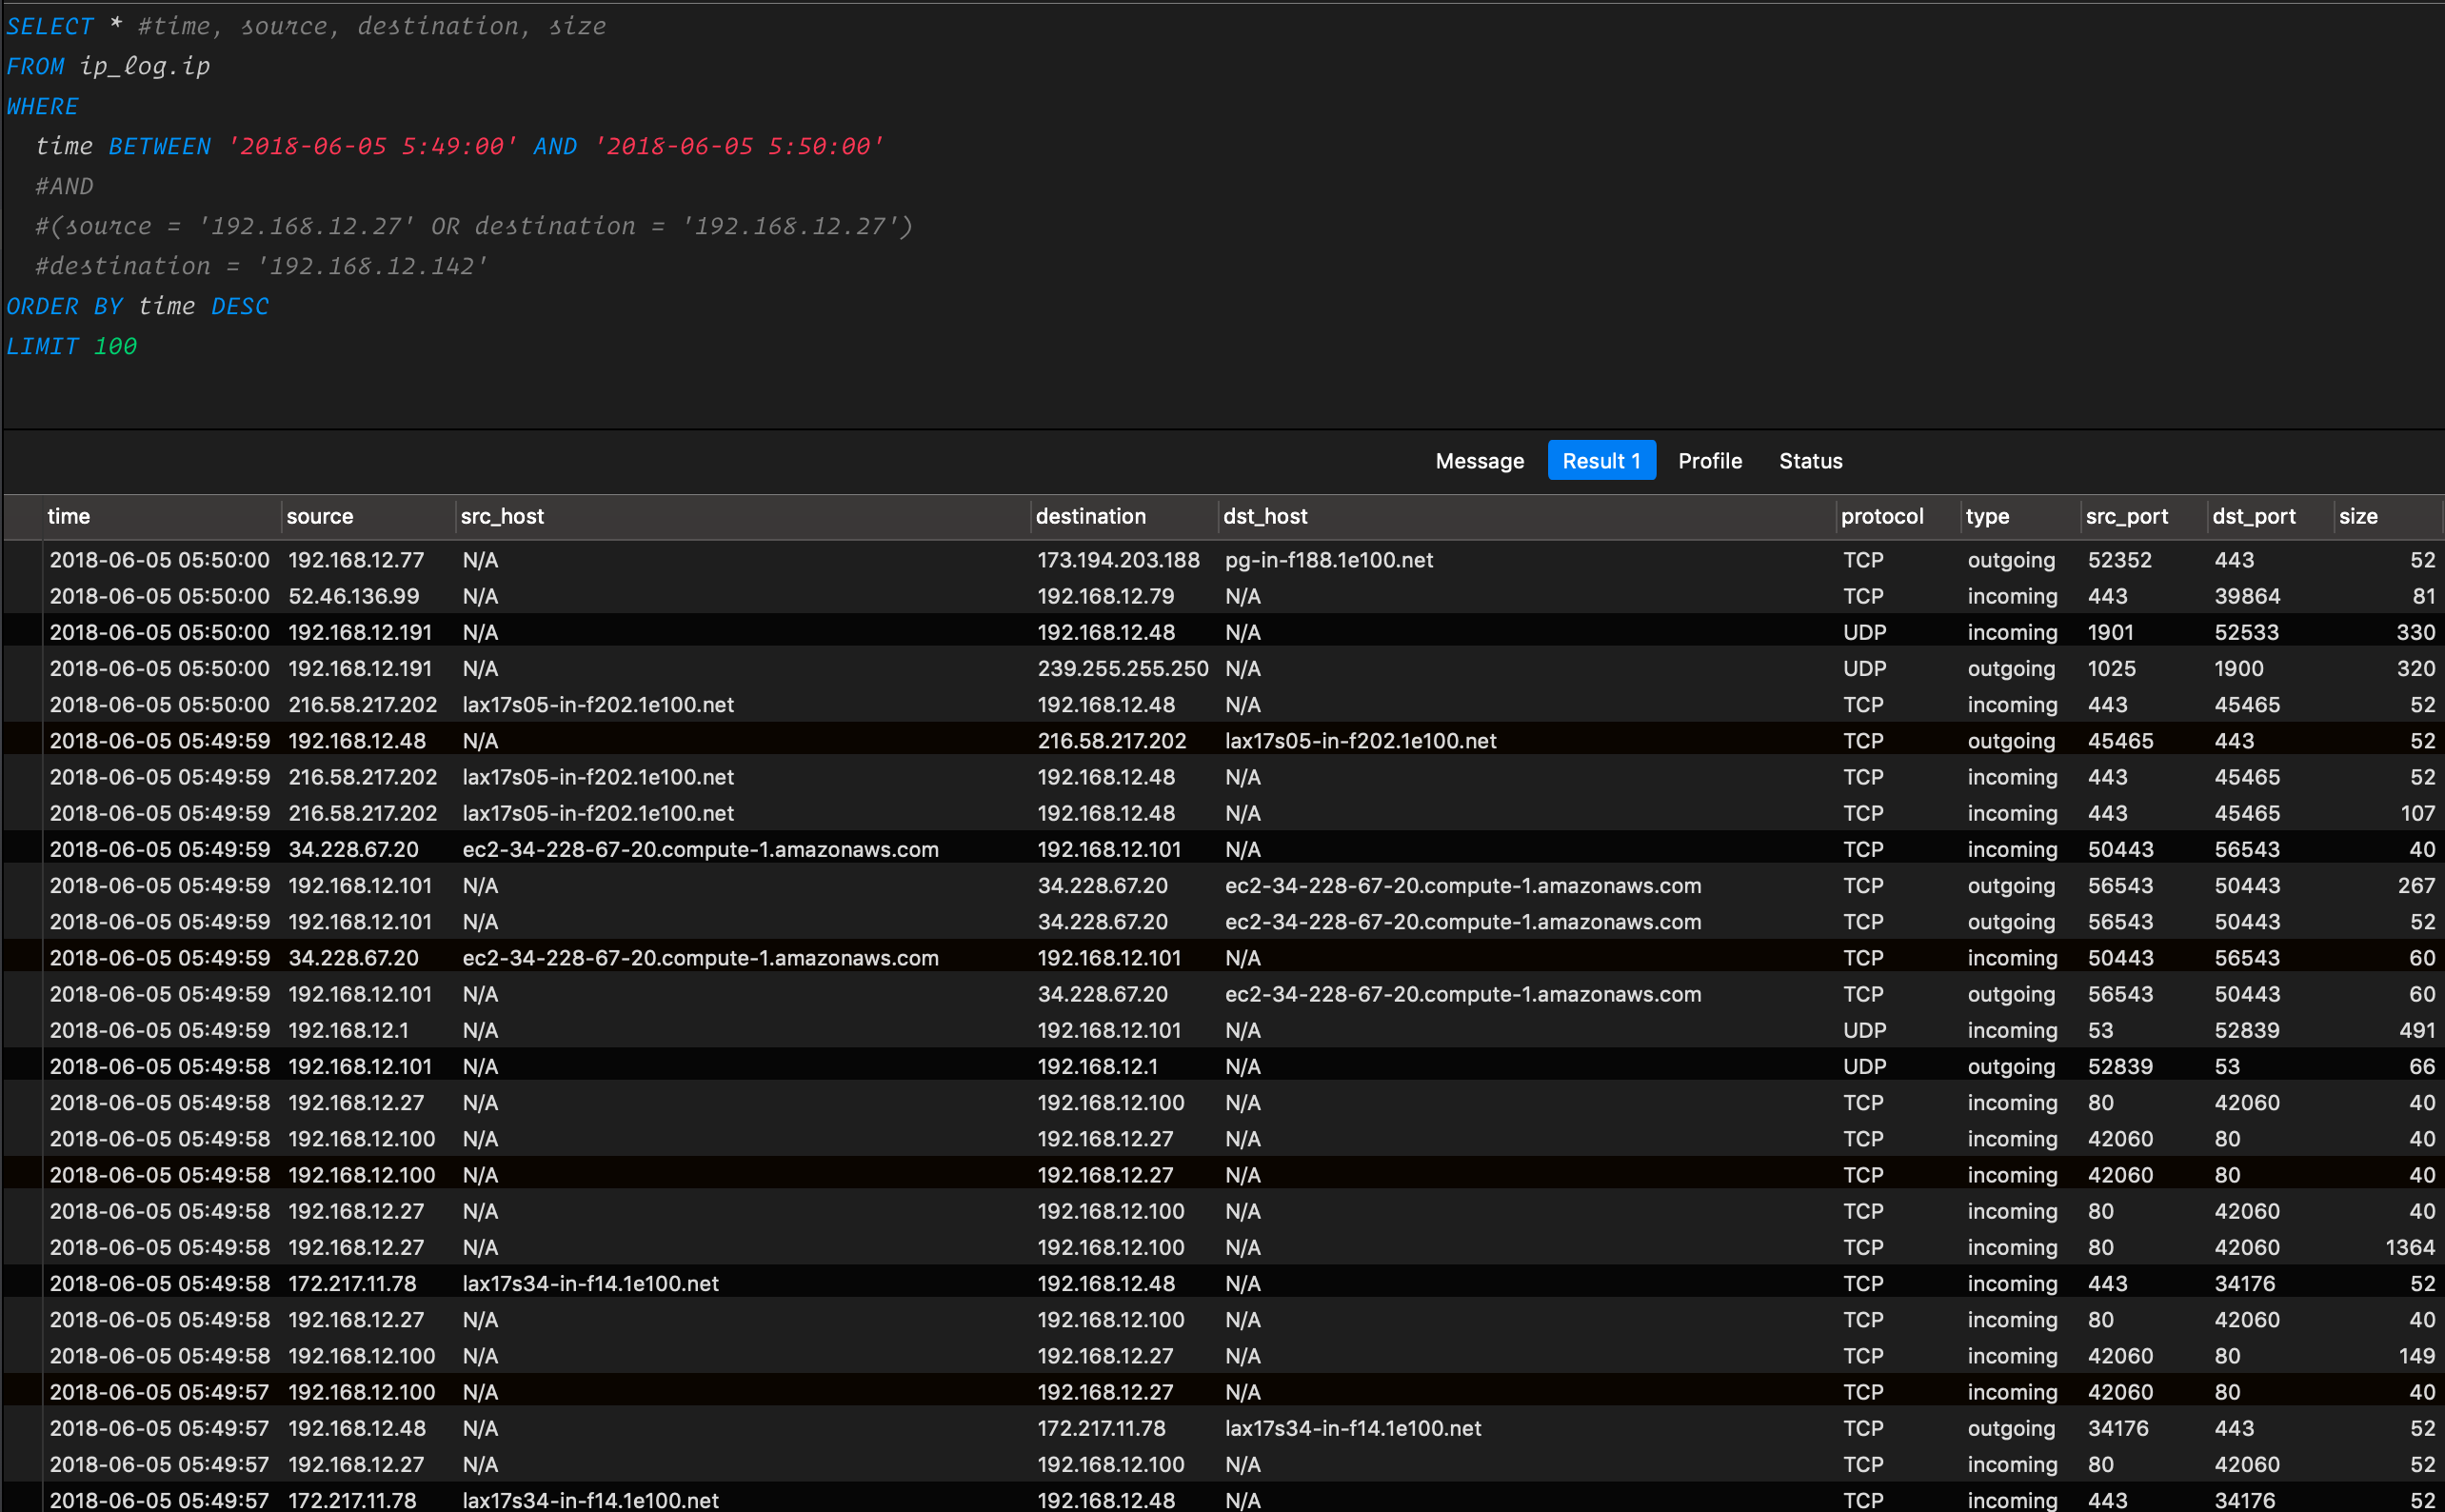
\includegraphics[width=1\textwidth]{figures/navicatNetworkQuery.png}
    \caption{Network query form database with Navicat.}
    \label{fig:navicatNetworkQuery}
\end{figure}
Within the power table, the name field is extracted from the name of the Wemo, which we manually name through the app. This can cause issues if the wrong device is connected to a Wemo. For example, the Echo Dot could've accidentally have been connected to the Wemo named Google home. There is no way to check for this besides manual examination, which we did after a few weeks, resetting all devices and causing a temporary void in power data in TIME RANGE. When we reset all devices, we also renamed some of the Wemos. For example, we changed "echoDot" to "Echo Dot". This way, all devices would follow the naming convention of separating words with spaces and capitalizing each word. A possible solution to this could've been to name the Wemo's by the IPs of the devices they connect to, but still, they are not static.

The sampling frequency for the power table is also low and missing some points. To handle missing points, interpolate points as shown in the \ref{realtimeIoTGrapher.py} section. There is nothing that can be done about the low sampling rate. This low sampling rate can cause some imprecise data through interpolation, some missing points may not have been a smooth change, drastic changes may have occurred that we may have missed.

\subsection{Usage Flow}

As previously stated, one of the goals of this paper is to create a data set that represents the baseline of normal network traffic and power usage. To do this, we used each IoT device at least twice a week for the 20 weeks of this research. To build a proper dataset that other people could use for research, we set up a list of things that we should do for each device at a minimum when interfacing with it. While doing this, we would log what the activities into a Google Sheets file so that these events could be correlated to entries in the database, giving context when looking back on this data. For example, if someone were to look at the database and notice that the power and network traffic was high for 3 minutes, they could look at our logs and see that the device was streaming music for those 3 minutes and assume that it was normal usage.

When logging events into the Google sheets, we include the start, end time, name of the device(s), action performed, and any individual notes. When naming the devices, we used the same naming as we did for the Wemos in order to maintain consistency and correlations from the log to the database. Because we manually enter entries through a Google sheet. An example of entries into the table is shown below in table\ref{tab:events}.

\begin{table}[H]
    \centering
    \caption{Event Log Excerpt}
    \begin{tabular}{@{}lllll@{}}
        \toprule
        Date & Start Time & End Time & Device & Event \\ \midrule
        5/25/2018 & 12:44:42 & 12:47:04 & Home Mini & Ask for news \\
        5/25/2018 & 12:55:07 & 12:56:37 & Echo Dot & Ask for news \\
        5/25/2018 & 12:55:57 & 12:56:17 & Echo Show & Ask for weather \\
        5/25/2018 & 12:56:44 & 13:03:07 & Home Mini & Play music \\ \bottomrule
        \end{tabular}
    \label{tab:events}
\end{table}

In the following subsections, we will explain the script created to automate the event logging portion of the research. Then we will follow up by explaining the specific procedure we ran each group of IoT devices through whenever we interfaced with them

\subsubsection{Google Sheets Script}

Logging information into the spreadsheet is a tedious task, especially when trying to analyze each device while running tasks on them. This can lead to poorly formatted entries. To minimize this as much as possible, we wrote a script to automatically populate the start time, end time, and date when entering entries. The code for the script can be shown below in listing~\ref{lst:sheetScript}.

\begin{lstlisting}[language=C,label={lst:sheetScript},caption={Open and Read from a Socket},captionpos=b]
function onEdit() {
  var s = SpreadsheetApp.getActiveSpreadsheet().getSheetByName("Event Log");
  var r = s.getActiveCell();
  var c = r.getColumn();

  if( c == 4 || c == 5) { // checks the column
    var dateCell = r.offset(0, -3);

    if( dateCell.getValue() === '' ) {// is empty?
      var startTimeCell = r.offset(0, -2);

      // fill in the start time and date
      var date = new Date();
      dateCell.setValue(date);
      startTimeCell.setValue(date.toLocaleTimeString());
    }
  }

  if( c == 6 ) { // checks that the description is being entered
    // if so fill in the end time
    var endTimeCell = r.offset(0, -3);

    if ( endTimeCell.getValue() === '' ) {
      endTimeCell.setValue(new Date().toLocaleTimeString());
    }
  }
}
\end{lstlisting}

\subsubsection{Smart Speakers}

Within the smart speakers' section, we include the Google Home, Echo Dot, Eufy Genie, and Echo Show. Whenever interfacing with these devices, we made sure to at least query for the weather and the news. The specific phrases we would use would be "<wakeword> what's the weather" and "<wakeword> what's the news". Then we would also make sure to set a reminder for a random task in a random timeframe. Then we would mute the devices for a few minutes. We muted these devices to see if they would still be listening if we said the wake word.

\subsubsection{Video Game Consoles}

Within the video game consoles section, we include the Xbox One and Nintendo Switch. When interfacing with these devices, we made sure to play a game on the device for at least 15 minutes. Every week, we would also browse for games on the game store and download free demos.

Afterward, we would turn off the Xbox and put the Nintendo Switch into sleep mode. The Nintendo Switch could not be put to sleep when docked, only when disconnected from the dock.

\subsubsection{Media Players}

Within the Media Players section, we include the Roku Express, Chromecast, and Amazon Firestick. When interfacing with these devices, we made sure to watch youtube for at least one video or 3 minutes.

For the Chromecast, we cycled through different devices to cast videos from in which included the Ipad and the Chromebook. We wanted to get varied data in case the Chromecast prioritized streaming from different devices.

\subsubsection{Tablets}

Within the tablets, we include the Samsung Galaxy Tablet and the IPad.

In this experimental setup, we used the tablets less so for investigative purposes, but more so that we can set up and interface with other devices. These devices are less IoT devices and more full-fledged computers. Thus they would have widely varied network patterns that would be difficult to track.

We mainly used these IPads to set up the WeMos and any device that had to be connected to a SmartHub. It was also used for controlling or changing the names of the WeMos through the app if necessary and for setting up the security camera.

However, regardless, we still tracked the data and had a small set list of things to do on these devices. We used each tablet to browse the web, watch YouTube, and use various apps.

\subsubsection{Security Camera}

The only security camera we worked with was the Eray Security Camera.

Whenever interfacing with this device, we used the device under the app (NVAS2) in the IPad for at least 2 minutes. Usage includes streaming video from the camera to tablet and viewing it. We also controlled the camera through the app through pan and tilt commands. When done experimenting with the security camera, we disconnected the tablet from the camera by using the "end stream" button in the NVAS2 app on IPad.

\subsection{realtimeIoTGrapher.py}
\label{realtimeIoTGrapher.py}

In this section, we will talk about further automation when researching Network and Power patterns. When analyzing the power and network for a particular device, we can only see so much when looking straight at the database entries. Even when filtering by device or time, we can only catch text but cannot visualize any patterns. To resolve this, we graphed the data into Google Sheets and graphed it. Seeing a graph made analysis and detection of patterns much easier. The tables and formulas are shown in figure\ref{fig:excelLogging}. This process was tedious and time-consuming. We had to copy the data over after making a sequel query, extract unique time columns, then sum the size up at each unique time frame. So we looked to optimize it.

The result was the realtimeIoTgrapher. This python script would automatically form the graphs shown in figure \ref{fig:tvThroughput} when given the time range and the devices. This automation sped up the analysis process and provided extra features which we will explain in section \ref{Features}.

This python script leveraged the Plotly library, which, given data, will graph it onto a local web page for viewing. It comes with many useful tools for further analysis and can be extended to run on a public web page for public viewing.

When we release this database to the public, we hope to complement it with this software so that researchers view the power and network information of any/all of the devices at a glance. At which point, we can set up a public website to host this software so that anyone can view the data at any time.

\begin{figure}[H]
    \centering
    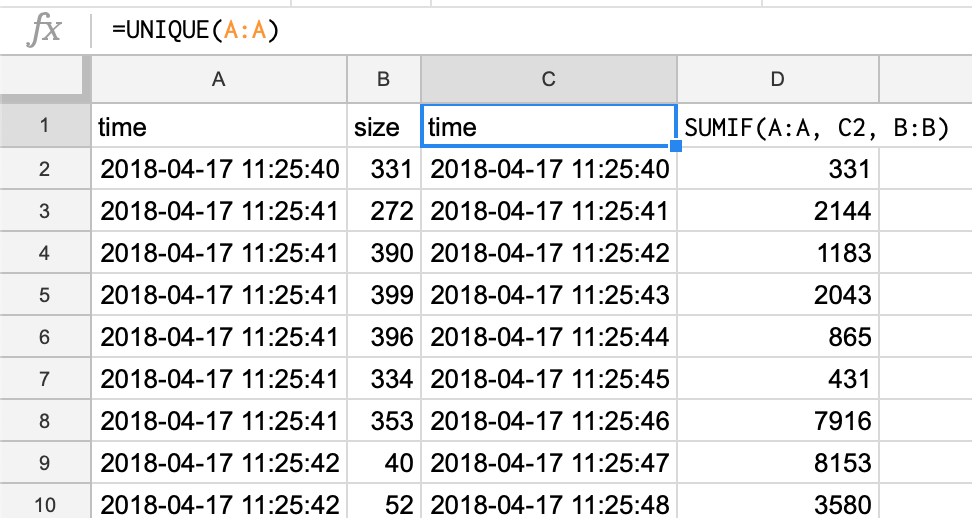
\includegraphics[width=1\textwidth]{excelLogging}
    \caption{Manual Analysis of IoT devices in Google Sheets: Raw data shown in columns A and B are then formatted into columns C and D for Graphing}
    \label{fig:excelLogging}
\end{figure}

\begin{figure}[H]
    \centering
    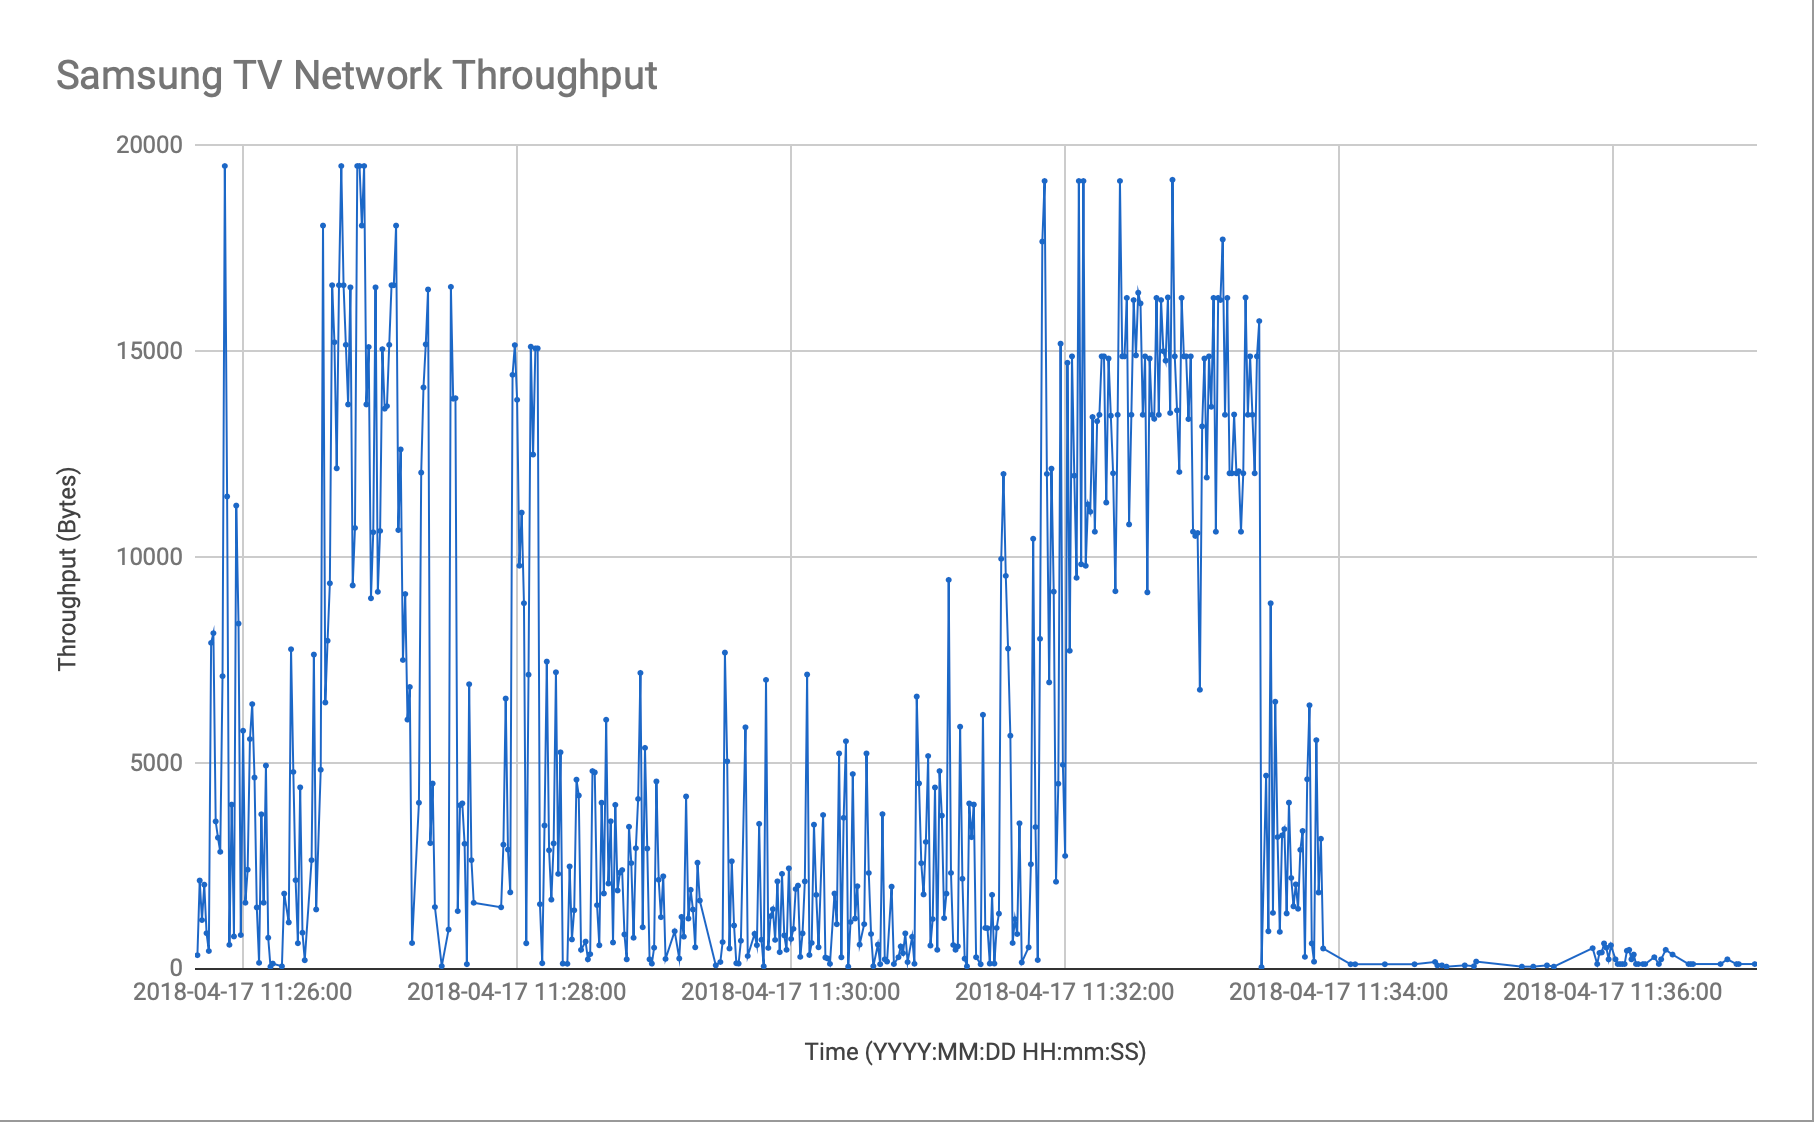
\includegraphics[width=1\textwidth]{figures/tvThroughput.png}
    \caption{Resulting graph of dataset shown in Figure \ref{fig:excelLogging}}
    \label{fig:tvThroughput}
\end{figure}

\subsubsection{Features}
\label{Features}

In this section, we will discuss the features that this RealTimeIoTGrapher (grapher) provides.

Firstly, at its core, this program automates the creation of the graph shown in figure \ref{fig:tvThroughput}. However, now, instead, we can specify a time range that the graph should be in, then we specify what devices we want to graph, and then the program will create the graph. It will show the power, input traffic, output network traffic, and the total network traffic over the time range specified as a line graph. The grapher will do this for all the devices specified.

On top of this core information, the grapher will also annotate the data by including a line denoting the average for each of the traces above over the time range that is currently displayed. It will also annotate the maximum and minimum values in the time range for each trace. Also, instead of a set time range, the grapher can also display this information in real time for an interval amount of time, updating every second.

The Plotly libraries also provide useful tools when displaying these IoT graphs. It is possible to zoom in and out the displayed graph, select specific traces for viewing, save the graph, and hover over data points to display the specific value. Finally, Plotly also provides a save feature that allows further editing of the graph so that it is formatted the way the user wants. There are many other features that the Plotly libraries provide, but these are the main ones used in our research.

\begin{figure}[H]
    \centering
    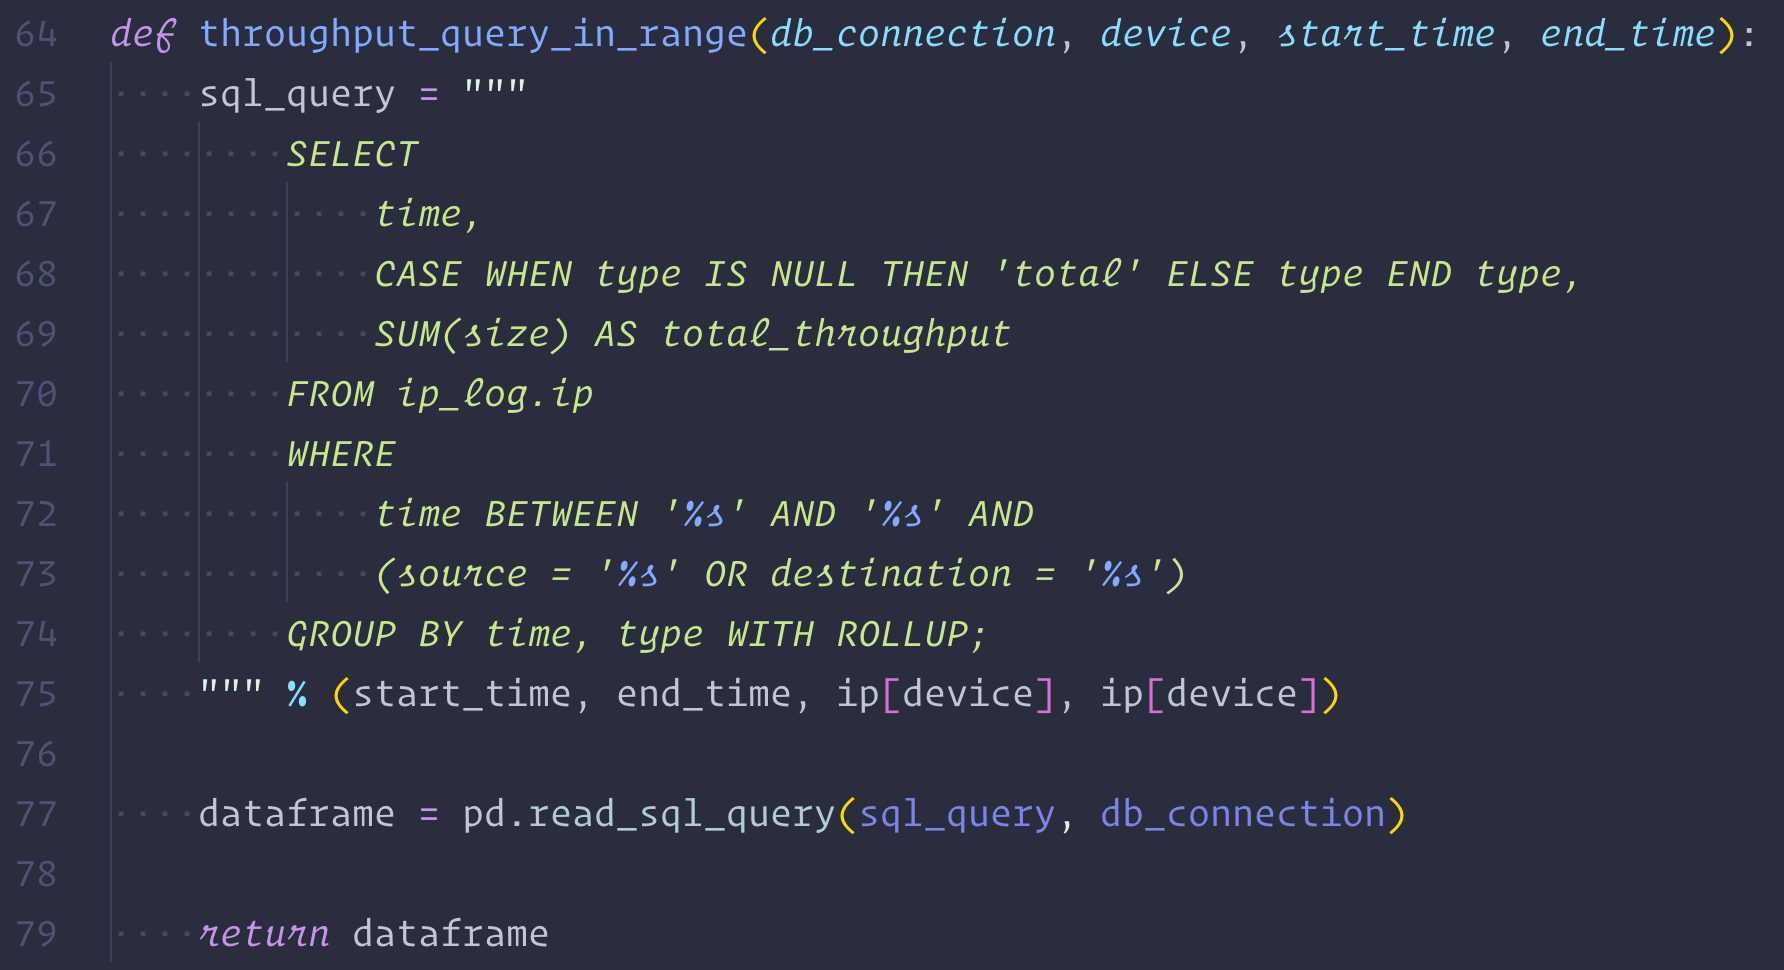
\includegraphics[width=1\textwidth]{figures/rollup.png}
    \caption{Efficient SQL query to obtain total Network throughput at each second}
    \label{fig:rollup}
\end{figure}

To reduce local computation, the grapher offloads work to the server through the SQL query. When querying for network data, it will perform a rollup in order to sum up the incoming and outcoming network throughput to obtain the total throughput. This roll-up query can is formatted as shown in \ref{fig:rollup}.

\begin{figure}[H]
    \centering
    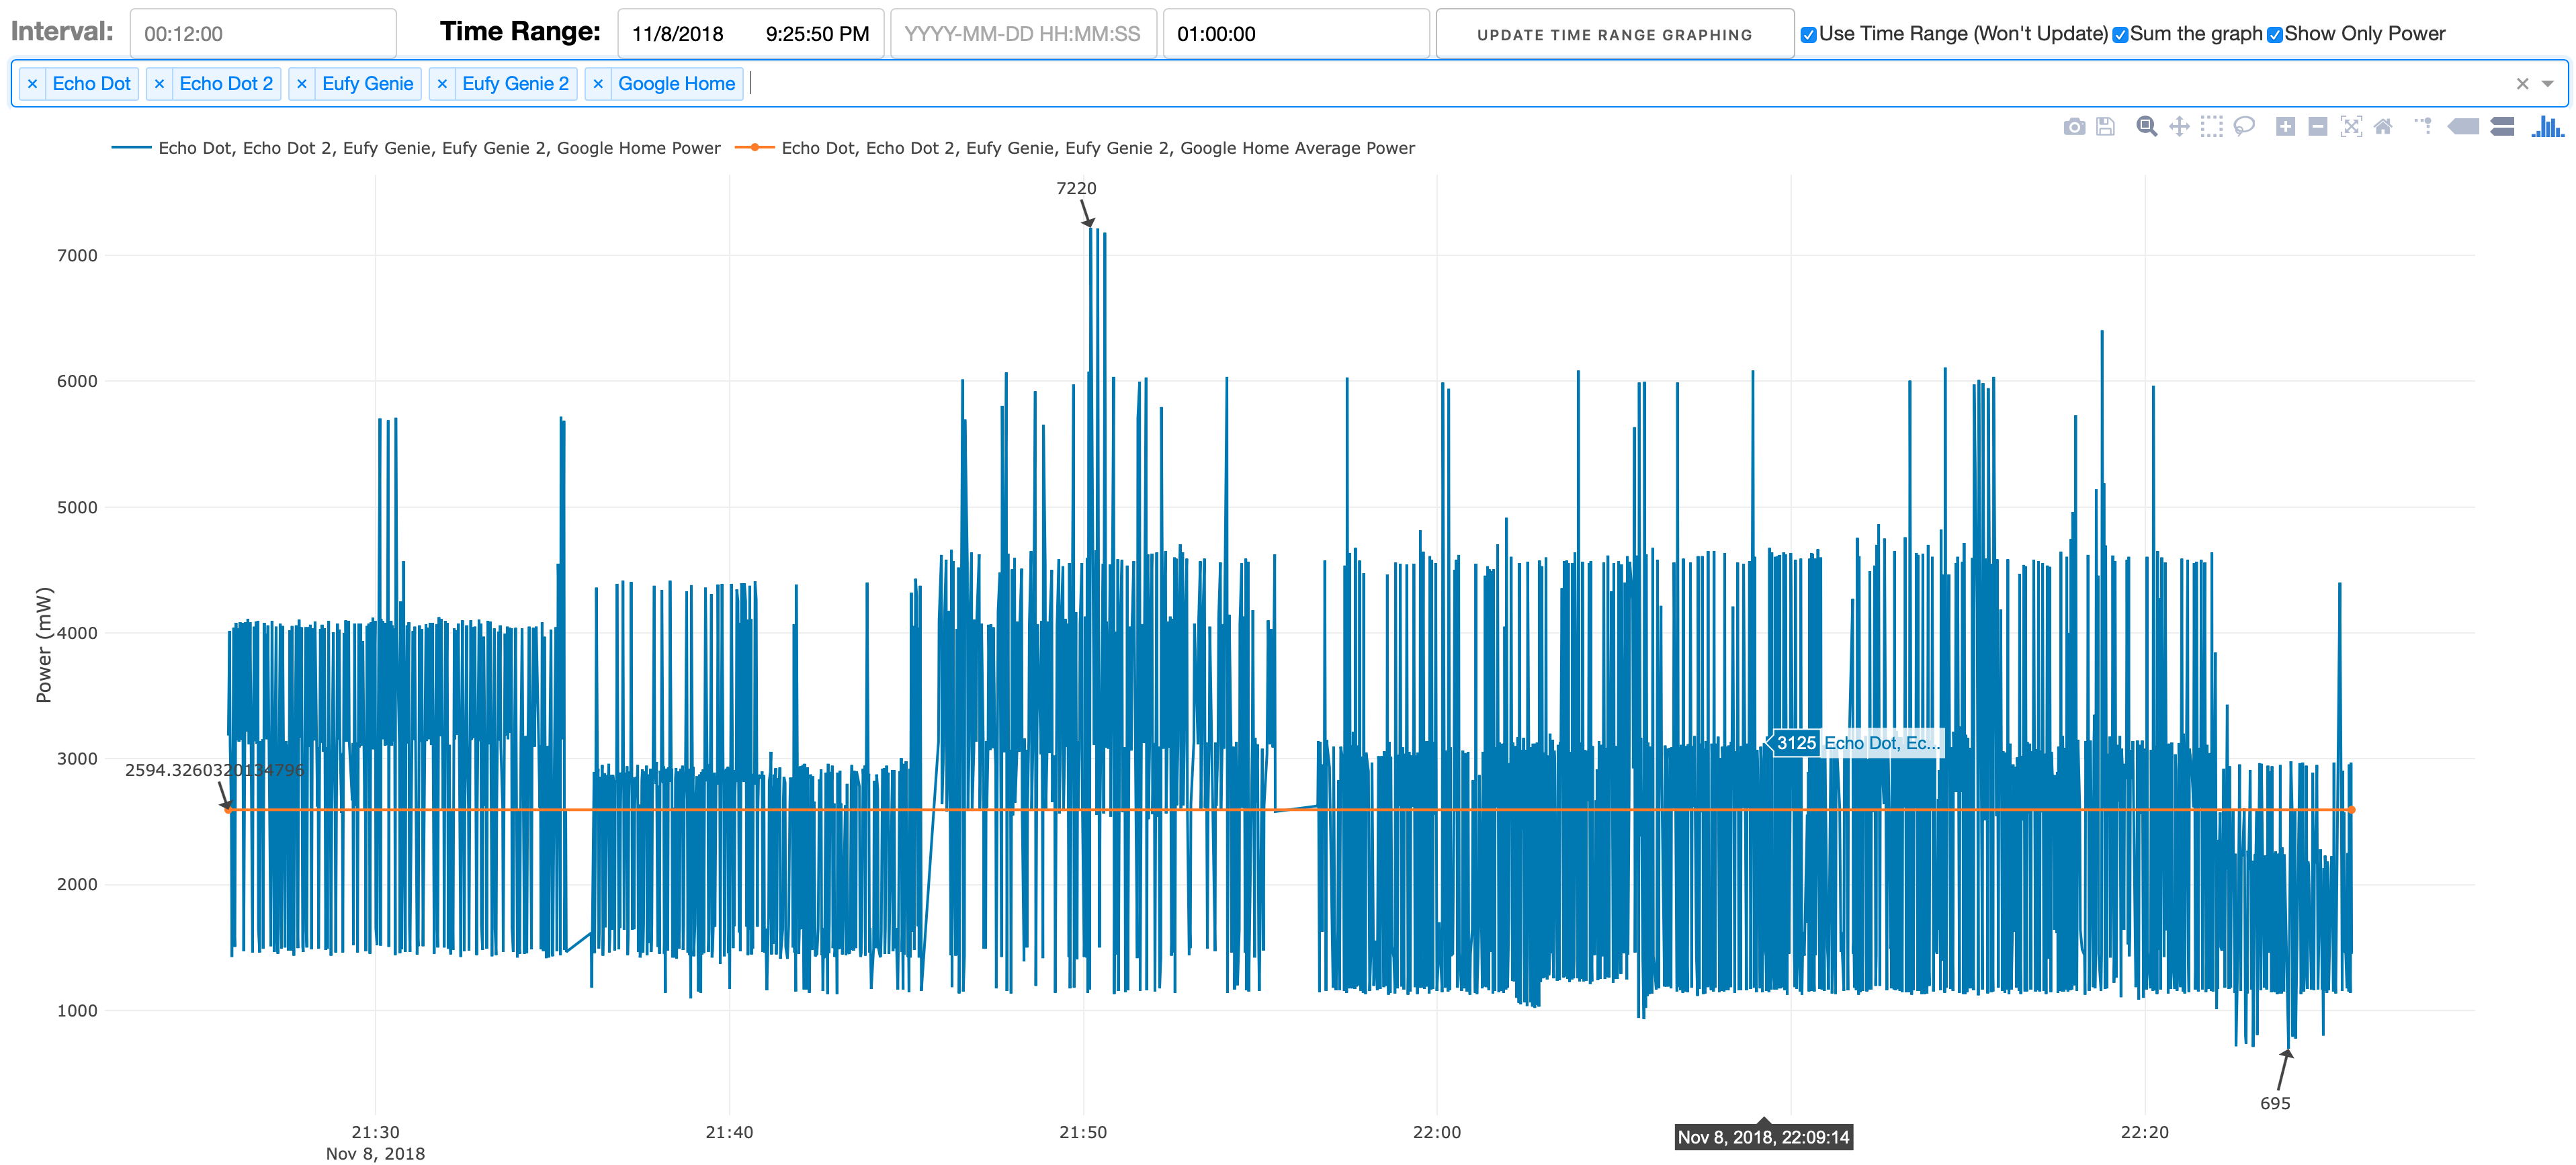
\includegraphics[width=1\textwidth]{figures/noninterpolated.png}
    \caption{Summed up power trace without interpolation.}
    \label{fig:noninterpolated}
\end{figure}

\begin{figure}[H]
    \centering
    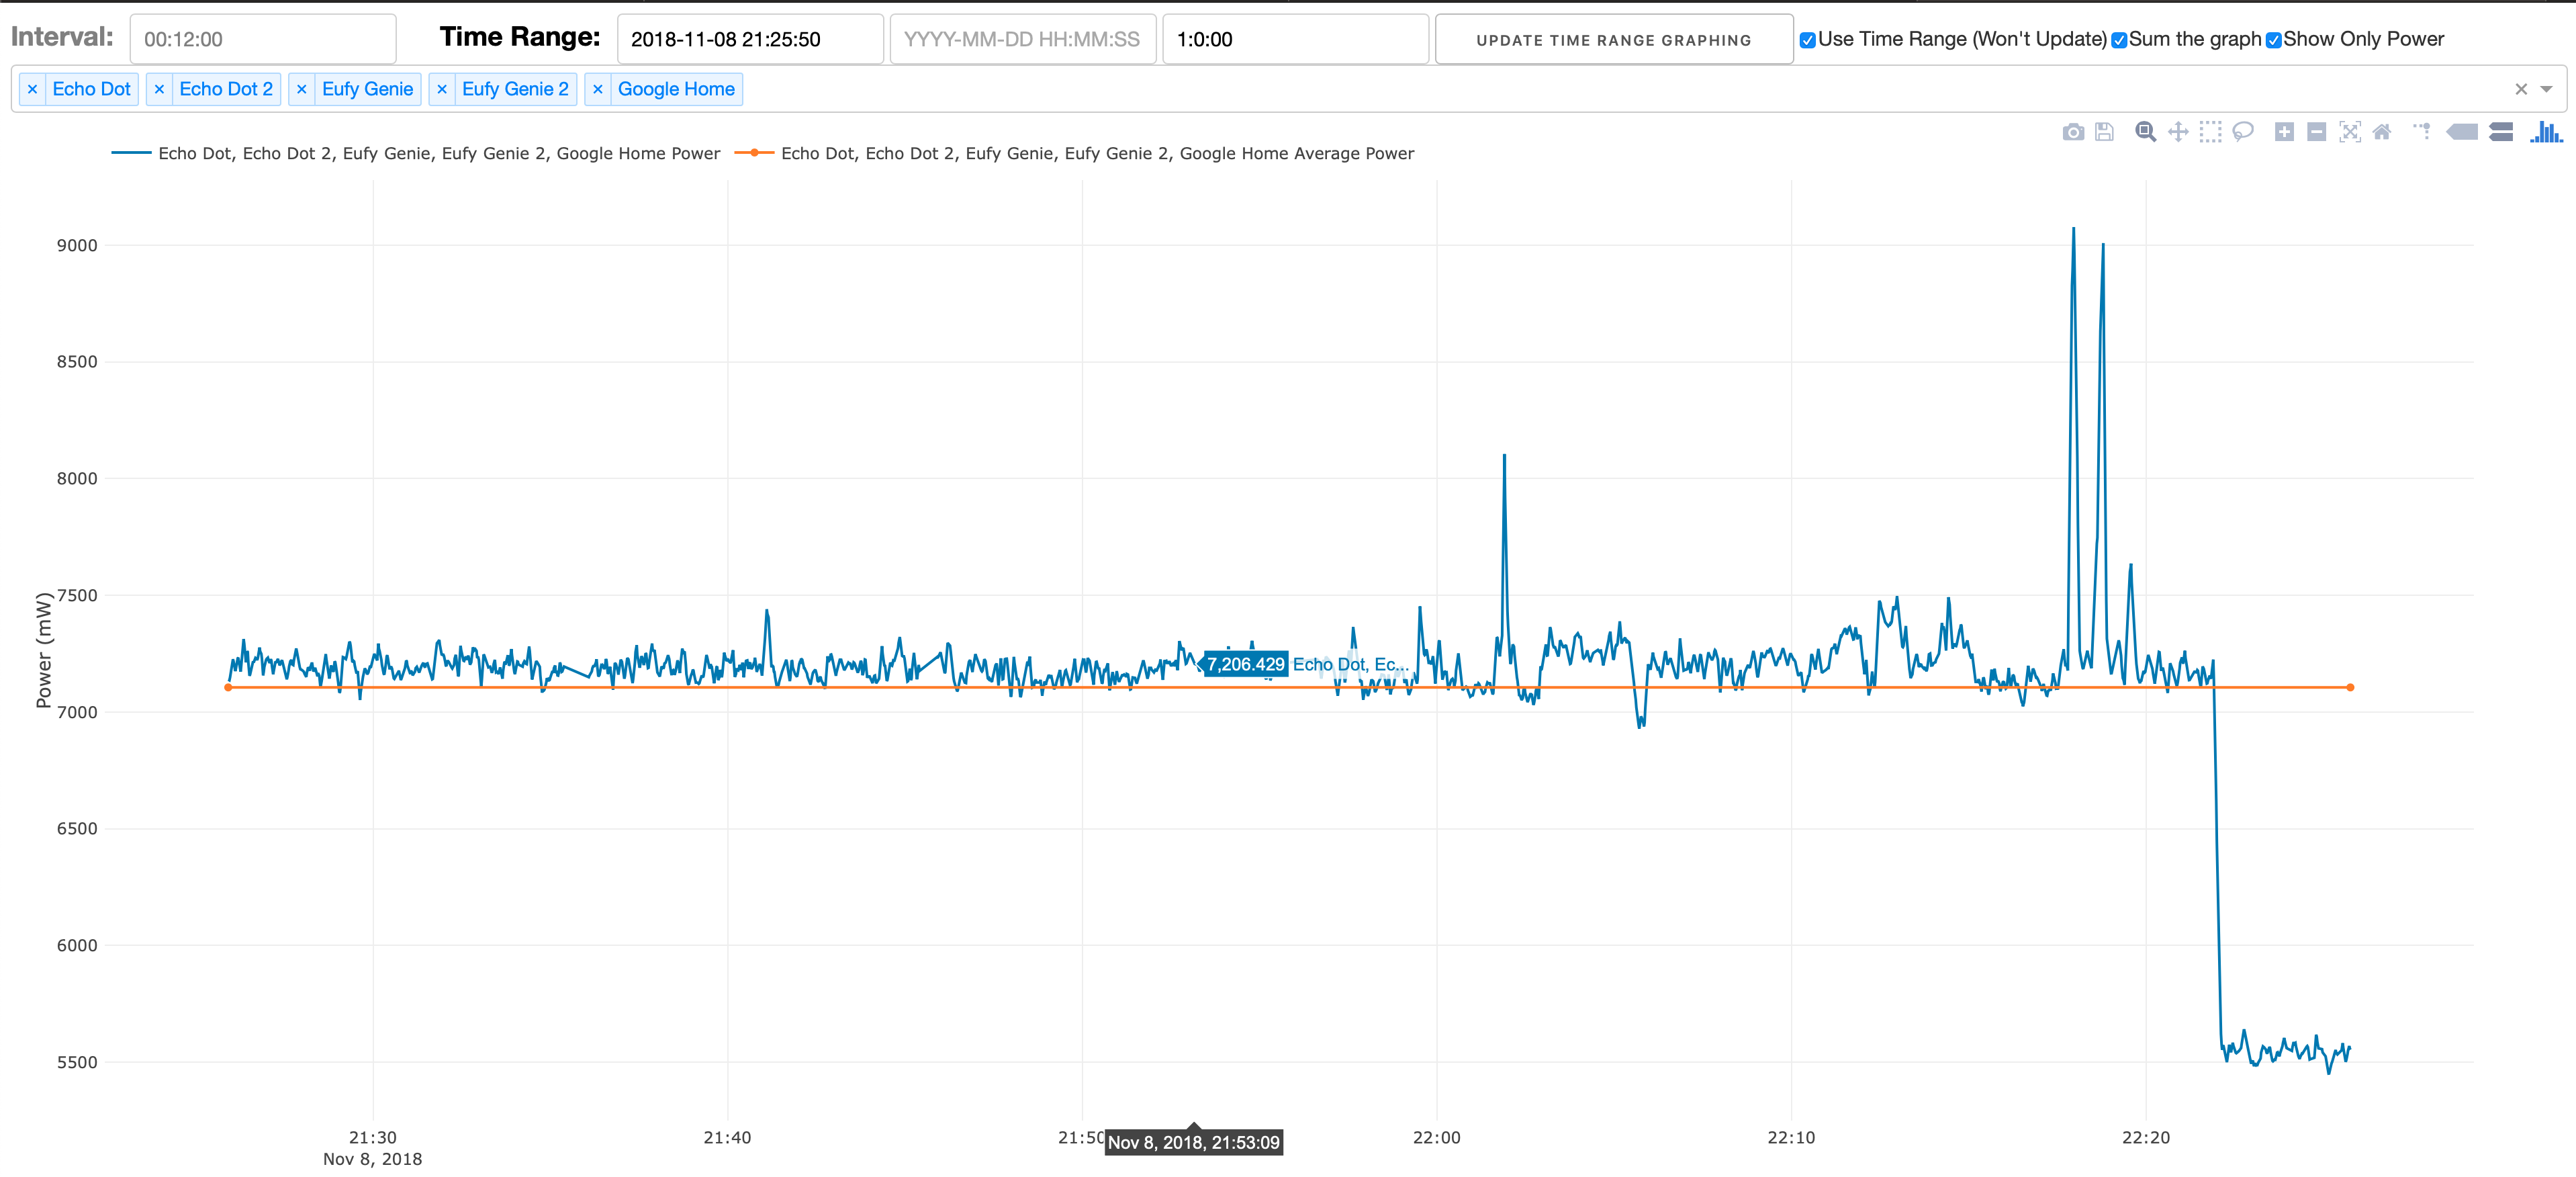
\includegraphics[width=1\textwidth]{figures/interpolated.png}
    \caption{Summed up power trace graph with interpolation.}
    \label{fig:interpolated}
\end{figure}

The grapher can also sum up all power traces into one single trace. Originally, when summing the graphs, it would add up the two Pandas data frames that are representing each trace and then graph that resultant trace, shown in figure \ref{fig:noninterpolated}. However, the Wemo doesn't always sample at every second. This is an issue if, at some second in time T, some device X has a power point, but the other device Y does not. The summation will count the empty data point in device Y at T as 0 and essentially take device X's data point as the sum. Device Y does not use 0 power at time T but doesn't have a data point for that time. So to solve this, we interpolated data for every second for each device before summing their data frames up, with a builtin Pandas feature. After using interpolation, the same time summed graph looks like figure \ref{fig:interpolated}. It is now much more accurate.

\subsubsection{Why It is Useful}
As stated before, this tool is meant to be released as a complementary tool to our database. It has already been utilized by multiple researchers when interfacing with our database.

The realTimeIoTGrapher will helps analysis of the database at a glance and gives insight into each device in relation to the event log.  This tool created most of the images shown in section \ref{Results}. Many other researchers have used this tool as well to gain a surface understanding of the database. The grapher provides real-time or historical graphs on any device for individual analysis or comparison with little effort or time. Additional features from Plotly also provides an easy way to format the graph for presentations or papers.

The summation feature can simplify the graph and provide a more holistic view of power usage as a whole, making it easier to spot patterns. In this paper, the feature is also used to simulate the concept of a household's "powerline" where all energy usage would be summed up into one power meter.

\subsubsection{Limitations}
As this tool was created entirely for research purposes in a constrained time frame, there are some edge cases that it fails to handle.

Every once in a while, since so many people are reading from the database, the database will have too many connections, at this point, the software will refuse to connect, and the grapher will not work.

The graphing tool also gets much slower when the time frame requested is much larger. We have noticed a slow down for queries in time frames longer than 7 hours. In the static graphing mode, it will slow down before graphing the information. However, in real time graphing mode, the tool will make many slow queries, eventually causing too many connections to the database and undefined behavior.

Because the IP addresses of the devices connected to the database are not static, they will change every once in a while. The Wemo names have also been changed a few times throughout this research for clarity purposes. The graphing tool uses a lookup table that maps the IP address of the device to the corresponding name given to the Wemos. Because we manually create the lookup table, when any of these fields change, the graphing tool will not be able to find the device and will not graph the devices information. In some cases, this situation is handled, and the graphing tool will ignore them. However, in some cases, the graphing tool will crash and require restarting. To solve this, manually change the IP addresses defined in the lookup table in line 23-39 shown in figure\ref{fig:ipLookup} below and increment/decrement the value of the IP a few times. In our experience, we at most had to change the IP up 3, but never more than that. This is just a guess and check method.

However, to figure out the new IP address for the table, we have to perform a SQL query in the time frame that a particular device is doing something, and manually examine to see which IP has the highest network throughput. With this method, we had to ensure only one device was in use so that an IP address for another device would not be confused for the current device. To change the corresponding name, check the device inventory excel sheet for a possibly updated naming scheme.

\begin{figure}[H]
    \centering
    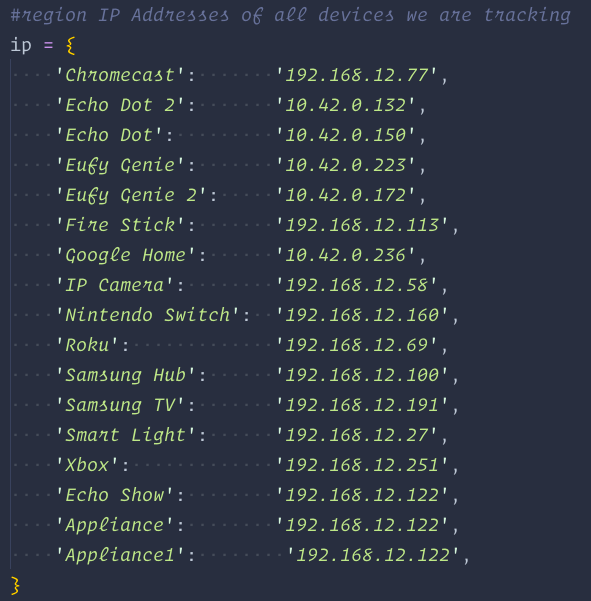
\includegraphics[width=1\textwidth]{figures/ipLookup.png}
    \caption{IP lookup table in real time iot grapher}
    \label{fig:ipLookup}
\end{figure}

\subsubsection{How To Install and Run}
To install and run this analysis tool, follow the instructions at the GitHub site:   \href{https://github.com/nealhnguyen/RealTimeIoTGrapher}{github.com/nealhnguyen/realtimeiotgrapher}.

First, pull the code for this tool from git hub and install the dependencies in the requirements file through pip. At this point, the dependencies are set to run this code on python 2.7.

Next, a 'loginCredentials' file must be created containing the host, user, password, and database information. At which point, running 'python realTimeIoTGraph.py' will start the backend and display its current operation onto the terminal.

The link to the local IP address will contain the graphing tool. Clicking on that will open it onto the default browser for the computer.

\subsubsection{Usage Directions}
Once the software is running, the grapher can be viewed on a web browser as shown in figure \ref{fig:grapherUsage}. This section will describe each numbered element in the image.

\begin{figure}[H]
    \centering
    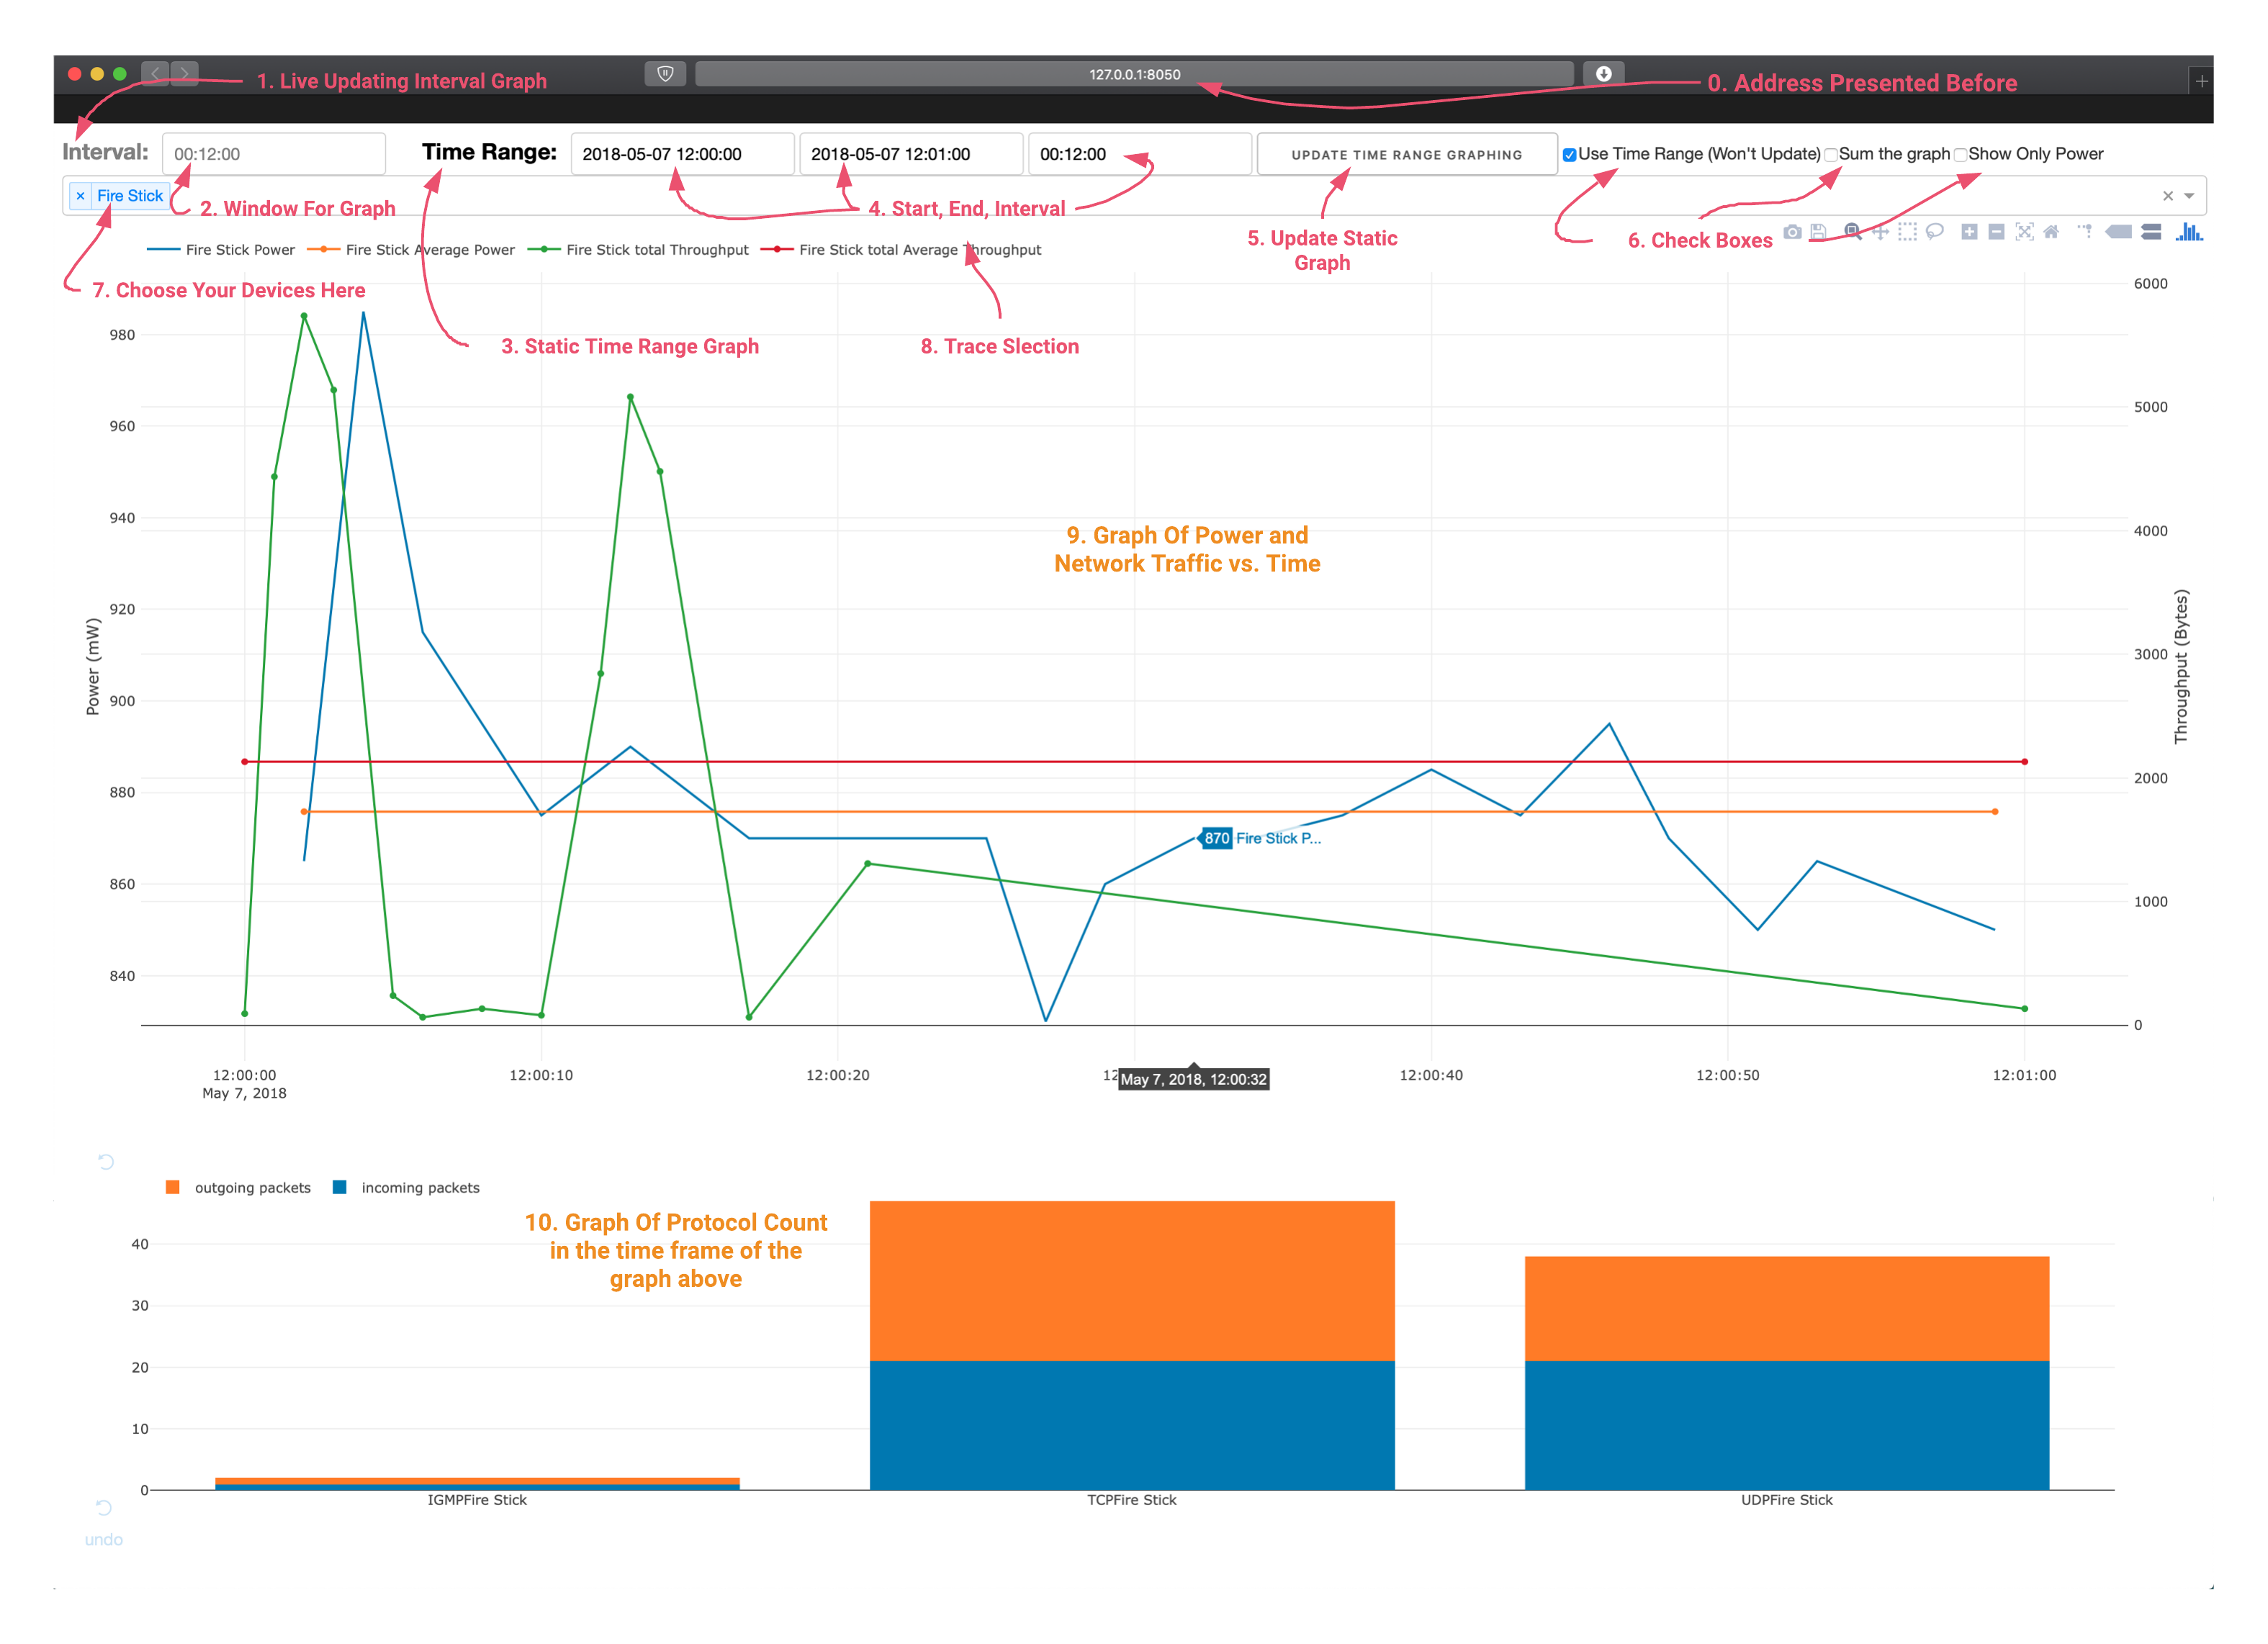
\includegraphics[width=1\textwidth]{figures/grapherUsage.png}
    \caption{RealTimeIoTGrapher usage image}
    \label{fig:grapherUsage}
\end{figure}

0. The local IP address presented in the terminal where the grapher is hosted.

1. The interval field and the text box next to it will be dark when the software is in live update mode.

2. The text box here relates to the live update feature of the graph. This is a time field, denoting the window of time the graph will display at a time while it updates. The format is HH:MM:SS where HH is the hour, MM is minutes, and SS is seconds.

3. The time range field and the four elements consecutively after it will be dark instead of grey when it is in static graph mode. In this state, the graphing tool will specify the network traffic and power information in the time window specified.

4. In these three text boxes, the time window for static graphing will be specified. The first box will be the start time, the second box will be the end time, and the last box will be the interval. To specify the time range, fill in any 2 of the three text boxes, and the graphing tool will infer the other number. If all three text boxes are filled, then the graphing tool will use the start and end time text box. To further explain, if the start time and interval are specified, then the window will be start time $\rightarrow$ start time + interval. If the end time and interval are specified, then the time window will be the end time - interval $\rightarrow$ end time.

5. This button causes the graph to update. After updating the time range in step 4, clicking this button will update the graph with the new time range.

6. The "Use Time Range" checkbox will toggle the software between live graph mode and static mode. The "Sum Graph" checkbox will sum up all power graphs into one. The "Show Only Power" checkbox will allow the grapher to avoid a SQL query for the network throughput, speeding up the process in case of pure power analysis.

7. This selection field specifies all the devices the software will create graphs. One, or many devices can be specified at a time. If too many devices are specified at a time, the software may run slow.

8. The traces shown can be selected or deflected to toggle its visibility.

9. This line graph will display the number of bytes sent through the network by a device going in, out, and in total. It will also show the power usage over time. Also, it will show the average value for a graph in the interval of the graph

10. This bar graph displays the spread of network traffic by protocol for each device. It displays the outgoing packets as orange and incoming packets as blue. It will display an individual bar graph for each device and protocol. Similarly, the traces can be clicked on to hide its visibility.
